% !TeX encoding = UTF-8

% 载入 SJTUThesis 模版
\documentclass[type=bachelor]{sjtuthesis}
% 选项
%   type=[doctor|master|bachelor|course],     % 可选(默认:doctor),论文类型
%   zihao=[-4|5],                             % 可选(研究生默认:-4,本科默认:5),正文字号大小
%   lang=[zh|en],                             % 可选(默认:zh),论文的主要语言
%   review,                                   % 可选(默认:关闭),盲审模式
%   [twoside|oneside]                         % 可选(默认:twoside),单双页模式

% 论文基本配置,加载宏包等全局配置
% !TEX root = ./main.tex

\sjtusetup{
  %
  %******************************
  % 注意:
  %   1. 配置里面不要出现空行
  %   2. 不需要的配置信息可以删除
  %******************************
  %
  % 信息录入
  %
  info = {%
    %
    % 标题
    %
    title           = {债权人会议系统设计与开发},
    title*          = {Creditor meeting system design and development},
    %
    % 标题页标题
    %   可使用“\\”命令手动控制换行
    %
    % display-title   = {上海交通大学学位论文\\ \LaTeX{} 模板示例文档},
    % display-title*  = {A Sample Document \\ for \LaTeX-based SJTU Thesis Template},
    %
    % 页眉标题
    %
    % running-title   = {示例文档},
    % running-title*  = {Sample Document},
    %
    % 关键词
    %
    keywords        = {债权人会议, 视频表决系统, 高并发, 实时系统},
    keywords*       = {Creditor's rights and meeting, Video voting system, High concurrency, Real-time},
    %
    % 姓名
    %
    author          = {王\quad{}浩\quad{}宇},
    author*         = {Mo Mo},
    %
    % 指导教师
    %
    supervisor      = {吴\quad{}刚},
    supervisor*     = {Prof. Mou Mou},
    %
    % 副指导教师
    %
    % assisupervisor  = {某某教授},
    % assisupervisor* = {Prof. Uom Uom},
    %
    % 学号
    %
    id              = {5140719024},
    %
    % 学位
    %   本科生不需要填写
    %
    degree          = {工学硕士},
    degree*         = {Master of Engineering},
    %
    % 专业
    %
    major           = {软件工程},
    major*          = {A Very Important Major},
    %
    % 所属院系
    %
    department      = {电子信息与电气工程学院},
    department*     = {Depart of XXX},
    %
    % 课程名称
    %   仅课程论文适用
    %
    course          = {某某课程},
    %
    % 答辩日期
    %   使用 ISO 格式 (yyyy-mm-dd);默认为当前时间
    %
    % date            = {2014-12-17},
    %
    % 资助基金
    %
    % fund  = {
    %           {国家 973 项目 (No. 2025CB000000)},
    %           {国家自然科学基金 (No. 81120250000)},
    %         },
    % fund* = {
    %           {National Basic Research Program of China (Grant No. 2025CB000000)},
    %           {National Natural Science Foundation of China (Grant No. 81120250000)},
    %         },
  },
  %
  % 风格设置
  %
  style = {%
    %
    % 本科论文页眉 logo 颜色 (red/blue/black)
    %
    % header-logo-color = black,
  },
  %
  % 名称设置
  %
  name = {
    % bib               = {References},
    % acknowledgements  = {谢\hspace{\ccwd}辞},
    % publications      = {攻读学位期间完成的论文},
  },
}

% 使用 BibLaTeX 处理参考文献
%   biblatex-gb7714-2015 常用选项
%     gbnamefmt=lowercase     姓名大小写由输入信息确定
%     gbpub=false             禁用出版信息缺失处理
\usepackage[backend=biber,style=gb7714-2015]{biblatex}
% 文献表字体
% \renewcommand{\bibfont}{\zihao{-5}}
% 文献表条目间的间距
\setlength{\bibitemsep}{0pt}
% 导入参考文献数据库
\addbibresource{bibdata/thesis.bib}

% 定义图片文件目录与扩展名
\graphicspath{{figures/}}
\DeclareGraphicsExtensions{.pdf,.eps,.png,.jpg,.jpeg}

% 确定浮动对象的位置,可以使用 [H],强制将浮动对象放到这里(可能效果很差)
% \usepackage{float}

% 固定宽度的表格
% \usepackage{tabularx}

% 使用三线表:toprule,midrule,bottomrule。
\usepackage{booktabs}

% 表格中支持跨行
\usepackage{multirow}

% 表格中数字按小数点对齐
\usepackage{dcolumn}
\newcolumntype{d}[1]{D{.}{.}{#1}}

% 使用长表格
\usepackage{longtable}

% 附带脚注的表格
\usepackage{threeparttable}

% 附带脚注的长表格
\usepackage{threeparttablex}

% 算法环境宏包
\usepackage[ruled,vlined,linesnumbered]{algorithm2e}
% \usepackage{algorithm, algorithmicx, algpseudocode}

% 代码环境宏包
\usepackage{listings}
\lstnewenvironment{codeblock}[1][]%
  {\lstset{style=lstStyleCode,#1}}{}

% 物理科学和技术中使用的数学符号,定义了 \qty 命令,与 siunitx 3.0 有冲突
% \usepackage{physics}

% 直立体数学符号
\newcommand{\dd}{\mathop{}\!\mathrm{d}}
\newcommand{\ee}{\mathrm{e}}
\newcommand{\ii}{\mathrm{i}}
\newcommand{\jj}{\mathrm{j}}

% 国际单位制宏包
\usepackage{siunitx}[=v2]

% 代码块宏包
\usepackage{listings}
% 代码高亮宏包
\usepackage{xcolor}
\usepackage{color}
\definecolor{dkgreen}{rgb}{0,0.6,0}
\definecolor{gray}{rgb}{0.5,0.5,0.5}
\definecolor{mauve}{rgb}{0.58,0,0.82}
\lstset{frame=tb,
     language=Java,
     aboveskip=3mm,
     belowskip=3mm,
     showstringspaces=false,
     columns=flexible,
     basicstyle = \ttfamily\small,
     numbers=none,
     numberstyle=\tiny\color{gray},
     keywordstyle=\color{blue},
     commentstyle=\color{dkgreen},
     stringstyle=\color{mauve},
     breaklines=true,
     breakatwhitespace=true,
     tabsize=3
}

% 定理环境宏包
\usepackage{ntheorem}
% \usepackage{amsthm}

% 绘图宏包
\usepackage{tikz}
\usetikzlibrary{shapes.geometric, arrows}

% 一些文档中用到的 logo
\usepackage{hologo}
\newcommand{\XeTeX}{\hologo{XeTeX}}
\newcommand{\BibLaTeX}{\textsc{Bib}\LaTeX}

% 借用 ltxdoc 里面的几个命令方便写文档
\DeclareRobustCommand\cs[1]{\texttt{\char`\\#1}}
\providecommand\pkg[1]{{\sffamily#1}}

% 自定义命令

% E-mail
\newcommand{\email}[1]{\href{mailto:#1}{\texttt{#1}}}

% hyperref 宏包在最后调用
\usepackage{hyperref}

% 自动引用题注更正为中文
\def\equationautorefname{式}
\def\footnoteautorefname{脚注}
\def\itemautorefname{项}
\def\figureautorefname{图}
\def\tableautorefname{表}
\def\partautorefname{篇}
\def\appendixautorefname{附录}
\def\chapterautorefname{章}
\def\sectionautorefname{节}
\def\subsectionautorefname{小节}
\def\subsubsectionautorefname{小节}
\def\paragraphautorefname{段落}
\def\subparagraphautorefname{子段落}
\def\FancyVerbLineautorefname{行}
\def\theoremautorefname{定理}


\begin{document}

%TC:ignore

% 标题页
\maketitle
% 原创性声明及使用授权书
\copyrightpage
% 插入外置原创性声明及使用授权书
% \copyrightpage[scans/sample-copyright-old.pdf]

% 前置部分
\frontmatter

% 摘要
% !TEX root = ../main.tex

\begin{abstract}
  近年来,在疫情、新一代数字技术的快速发展以及国家对于数字化基础设施建设大力支持的影响下,各行各业都加快进行数字化变革。在破产领域中,债权人会议是破产程序中必不可少的一环,而由于现场会议召开的成本过高且十分受限于疫情,而传统会议系统又无法满足债权人会议需求,因此需要对债权人会议业务的全面数字化。
  
  本文针对债权人会议人数多、请求在短时间内密集、实时性要求高的特点提出针对高并发场景、实时反映表决情况的债权人会议系统的设计与开发方案,结合相关法律知识,贴合债权人会议的现实业务,通过使用 Kafka 进行流量削峰解和使用 Redis 做高速缓存解决高并发情况下带来的问题,通过对实时后端的针对设计让债权人会议系统的实时性更强,使债权人会议的线上召开更为流畅。
  
  目前对债权人会议系统的研究十分匮乏,本文在法律业务数字化、债权人会议系统的设计开发、高并发架构针对设计、实时业务开发等方面提供了一定的参考价值。通过实验,本系统性能达到预期效果,Mongo 写入性能为本系统性能瓶颈,之后优化方向可以从此方面着手。
\end{abstract}

\begin{abstract*}
  In recent years, under the influence of the epidemic, the rapid development of a new generation of digital technology and the country's strong support for the construction of digital infrastructure, all industries are accelerating digital transformation. In the field of bankruptcy, creditors' meeting is an essential part of the bankruptcy process. However, due to the high cost of on-site meeting, which is very limited by the epidemic, and the traditional meeting system cannot meet the needs of creditors' meeting, it is necessary to fully digitize the creditors' meeting business.



  In view of the characteristics of large number of creditors' meetings, intensive requests in a short time and high real-time requirements, this paper proposes the design and development scheme of creditors' meeting system for high concurrent scenarios and real-time reflection of voting situation, and combines relevant legal knowledge to fit the realistic business of creditors' meetings. Through the use of Kafka flow peak cutting solution and the use of Redis cache to solve the problem of high concurrency, through the design of the real-time back-end so that the real-time creditor meeting system is stronger, so that the online creditor meeting is more fluent.



  At present, the research of creditor meeting system is very scarce. This paper provides some reference value in legal business digitization, creditor meeting system design and development, high concurrency architecture design, real-time business development and so on.Through the experiment, the system performance achieves the desired effect, and the Mongo write performance is the bottleneck of the system performance, and then the optimization direction can start from this aspect.
\end{abstract*}


% 目录
\tableofcontents
% 插图索引
\listoffigures*
% 表格索引
\listoftables*

%TC:endignore

% 主体部分
\mainmatter

% 正文内容
% !TEX root = ../main.tex

\chapter{绪论}
DevOps 这一理念最早



这是 \sjtuthesis 的sdfgh示例文档,基本上覆盖了模板中所有格式的设置。建议大家在使用模
板之前,除了阅读《\sjtuthesis\ 使用文档》,这个示例文档也最好能看一看。

\section{研究背景与意义}

\subsection{三级标题}

\subsubsection{四级标题}

Lorem ipsum dolor sit amet, consectetur adipiscing elit, sed do eiusmod tempor
incididunt ut labore et dolore magna aliqua. Ut enim ad minim veniam, quis
nostrud exercitation ullamco laboris nisi ut aliquip ex ea commodo consequat.
Duis aute irure dolor in reprehenderit in voluptate velit esse cillum dolore eu
fugiat nulla pariatur. Excepteur sint occaecat cupidatat non proident, sunt in
culpa qui officia deserunt mollit anim id est laborum.

\section{脚注}

Lorem ipsum dolor sit amet, consectetur adipiscing elit, sed do eiusmod tempor
incididunt ut labore et dolore magna aliqua. \footnote{Ut enim ad minim veniam,
quis nostrud exercitation ullamco laboris nisi ut aliquip ex ea commodo
consequat. Duis aute irure dolor in reprehenderit in voluptate velit esse cillum
dolore eu fugiat nulla pariatur.}

\section{字体}


上海交通大学是我国历史最悠久的高等学府之一,是教育部直属、教育部与上海市共建的全
国重点大学,是国家“七五”、“八五”重点建设和“211 工程”、“985 工程”的首批建
设高校。经过 115 年的不懈努力,上海交通大学已经成为一所“综合性、研究型、国际化”
的国内一流、国际知名大学,并正在向世界一流大学稳步迈进。

{\songti 十九世纪末,甲午战败,民族危难。中国近代著名实业家、教育家盛宣怀和一批
  有识之士秉持“自强首在储才,储才必先兴学”的信念,于 1896 年在上海创办了交通大
  学的前身——南洋公学。建校伊始,学校即坚持“求实学,务实业”的宗旨,以培养“第
  一等人才”为教育目标,精勤进取,笃行不倦,在二十世纪二三十年代已成为国内著名的
  高等学府,被誉为“东方MIT”。抗战时期,广大师生历尽艰难,移转租界,内迁重庆,
  坚持办学,不少学生投笔从戎,浴血沙场。解放前夕,广大师生积极投身民主革命,学校
  被誉为“民主堡垒”。}

{\heiti 新中国成立初期,为配合国家经济建设的需要,学校调整出相当一部分优势专业、
  师资设备,支持国内兄弟院校的发展。五十年代中期,学校又响应国家建设大西北的号
  召,根据国务院决定,部分迁往西安,分为交通大学上海部分和西安部分。1959 年 3月
  两部分同时被列为全国重点大学,7 月经国务院批准分别独立建制,交通大学上海部分启
  用“上海交通大学”校名。历经西迁、两地办学、独立办学等变迁,为构建新中国的高等
  教育体系,促进社会主义建设做出了重要贡献。六七十年代,学校先后归属国防科工委和
  六机部领导,积极投身国防人才培养和国防科研,为“两弹一星”和国防现代化做出了
  巨大贡献。}

{\kaishu 改革开放以来,学校以“敢为天下先”的精神,大胆推进改革:率先组成教授代
  表团访问美国,率先实行校内管理体制改革,率先接受海外友人巨资捐赠等,有力地推动
  了学校的教学科研改革。1984 年,邓小平同志亲切接见了学校领导和师生代表,对学校
  的各项改革给予了充分肯定。在国家和上海市的大力支持下,学校以“上水平、创一流”
  为目标,以学科建设为龙头,先后恢复和兴建了理科、管理学科、生命学科、法学和人文
  学科等。1999 年,上海农学院并入;2005 年,与上海第二医科大学强强合并。至此,学
  校完成了综合性大学的学科布局。近年来,通过国家“985 工程”和“211 工程”的建
  设,学校高层次人才日渐汇聚,科研实力快速提升,实现了向研究型大学的转变。与此同
  时,学校通过与美国密西根大学等世界一流大学的合作办学,实施国际化战略取得重要突
  破。1985 年开始闵行校区建设,历经 20 多年,已基本建设成设施完善,环境优美的现
  代化大学校园,并已完成了办学重心向闵行校区的转移。学校现有徐汇、闵行、法华、七
  宝和重庆南路(卢湾)5 个校区,总占地面积 4840 亩。通过一系列的改革和建设,学校
  的各项办学指标大幅度上升,实现了跨越式发展,整体实力显著增强,为建设世界一流大
  学奠定了坚实的基础。}

{\ifcsname fangsong\endcsname\fangsong\else[无 \cs{fangsong} 字体。]\fi 交通大学
  始终把人才培养作为办学的根本任务。一百多年来,学校为国家和社会培养了 20余万各
  类优秀人才,包括一批杰出的政治家、科学家、社会活动家、实业家、工程技术专家和医家,如江泽民wowowowowowowoow陆定一、丁关根、汪道涵、钱学森、吴文俊、徐光宪、张光斗、黄炎
  培、邵力子、李叔同、蔡锷、邹韬奋、陈敏章、王振义、陈竺等。在中国科学院、中国工
  程院院士中,有 200 余位交大校友;在国家 23 位“两弹一星”功臣中,有 6 位交大校
  友;在 18 位国家最高科学技术奖获得者中,有 3 位来自交大。交大创造了中国近现代
  发展史上的诸多“第一”:中国最早的内燃机、最早的电机、最早的中文打字机等;新中国
  第一艘万吨轮、第一艘核潜艇、第一艘气垫船、第一艘水翼艇、自主设计的第一代战斗
  机、第一枚运载火箭、第一颗人造卫星、第一例心脏二尖瓣分离术、第一例成功移植同种
  原位肝手术、第一例成功抢救大面积烧伤病人手术等,都凝聚着交大师生和校友的心血智
  慧。改革开放以来,一批年轻的校友已在世界各地、各行各业崭露头角。}

{\ifcsname lishu\endcsname\lishu\else[无 \cs{lishu} 字体。]\fi 截至 2011 年 12
  月 31 日,学校共有 24 个学院 / 直属系(另有继续教育学院、技术学院和国际教育学
  院),19 个直属单位,12 家附属医院,全日制本科生 16802 人、研究生24495 人(其
  中博士研究生 5059 人);有专任教师 2979 名,其中教授 835 名;中国科学院院士 15
  名,中国工程院院士 20 名,中组部“千人计划”49 名,“长江学者”95 名,国家杰出
  青年基金获得者 80 名,国家重点基础研究发展计划(973 计划)首席科学家 24名,国
  家重大科学研究计划首席科学家 9名,国家基金委创新研究群体 6 个,教育部创新团队
  17 个。}

{\ifcsname youyuan\endcsname\youyuan\else[无 \cs{youyuan} 字体。]\fi 学校现有本
  科专业 68 个,涵盖经济学、法学、文学、理学、工学、农学、医学、管理学和艺术等九
  个学科门类;拥有国家级教学及人才培养基地 7 个,国家级校外实践教育基地 5个,国
  家级实验教学示范中心 5 个,上海市实验教学示范中心 4 个;有国家级教学团队 8个,
  上海市教学团队 15 个;有国家级教学名师 7 人,上海市教学名师 35 人;有国家级精
  品课程 46 门,上海市精品课程 117 门;有国家级双语示范课程 7 门;2001、2005 和
  2009 年,作为第一完成单位,共获得国家级教学成果 37 项、上海市教学成果 157
  项。}

% !TEX root = ../main.tex

\chapter{背景介绍}

数字化是信息技术发展的高级阶段,是数字经济的主要驱动力,随着新一代数字技术的快速发展,各行各业利用数字技术创造了越来越多的价值,这又推动了各行业加快进行数字化变革。本章从对律师行业破产领域的债权会议全面数字化的研究背景意义出发,系统阐述国内外研究最新研究成果。

\section{研究背景与意义}

\subsection{研究的背景}
本文提到的数字化主要是利用数字技术,对具体业务、场景的数字化改造。数字技术革命推动了人类的数字化变革。人类社会的经济形态随着技术的进步不断演变,农耕技术开启了农业经济时代,工业革命实现了农业经济向工业经济的演变,如今数字技术革命,推动了人类生产生活的数字化变革,孕育出一种新的经济形态——数字经济,数字化成为数字经济的核心驱动力。数字技术的不断完善让数字化的价值得到充分发挥。近年来,物联网、云计算、人工智能等各类数字技术不断更新,从实验向实践,逐渐工业化,形成了完整的数字化价值链,在各个领域实现应用,推动了各个行业的数字化,为各行业不断创造新的价值。数字基础设施快速发展推动数字化的应用。近年来,我国不断加快数字基础设施建设,推进工业互联网、人工智能、物联网、车联网、大数据、云计算、区块链等技术集成创新和融合应用,让数字化应用更加广泛深入到社会经济运行的各个层面,推动数字经济的发展。

律师行业作为一个传统行业,目前大部分还处于传统的手工业时代,信息靠纸质材料收集整理,存储靠库房堆积,十分影响效率。如今正处疫情期间,线下办公的方式受到了极大的限制,而业务不会因为限制的存在而减少,大量的业务堆积带来了极大的不便,律师行业的数字化变革迫在眉睫。

而在破产领域中,会议和表决的意义十分重大,决定着一个破产项目的走向,为了实现破产业务的数字化转型,专门设计针对破产项目表决的会议系统是必不可少的。企业破产项目债权人很容易高达千人级别甚至万人级别,如果同时进行多场会议,且在同一时间段进行表决的情况下,并发量将极大的提升,对服务器造成极大的压力,因此需要设计开发专门针对高并发情况下的会议表决系统。

\subsection{研究的意义}
破产领域的债权会议全面数字化的研究意义主要有以下三点。

一是由于受新冠肺炎疫情影响,通过网络形式召开债权人会议成为管理人的主要选择。网络债权人会议所代表的破产案件线上化操作的优势是非常明显的——这种优势不仅体现在疫情期间,线上化操作无论程序设计还是设备使用,更加简便快捷和规范高效,代表破产业务未来的工作趋势。网络债权人会议是在网络时代下,利用网络技术对债权人会议召开方式的革新,有利于提高工作效率,有利于更好保障债权人权利。但网络债权人会议有别于传统债权人会议,产生了许多新的问题需要解决。债权会议系统有别于常规的会议系统,和破产法律紧密挂钩,常规的会议系统并不适用,因此需要设计开发针对性的债权会议系统。

二是数字化以数据为主要生产要素,将企业中所有的业务、生产、营销、客户等有价值的人、事、物全部转变为数字存储的数据,形成可存储、可计算、可分析的数据、信息、知识,并和企业获取的外部数据一起,通过对这些数据的实时分析、计算、应用可以指导企业生产、运营等各项业务。而每一次的债权会议都能产生大量的数据,这些数据可以产生极大的经济价值,因此需要保证对这些数据的存储的可靠性。

三是近年来随着计算机技术和网络技术的迅速崛起,互联网日渐深刻的在改变着人们的生产生活方式。互联网的发展带来了需求的激增、技术上的压力,系统架构也因此不断的演进、升级、迭代。从单一应用,到垂直拆分,到分布式服务,到 SOA ,以及现在火热的微服务架构。虽然解决了大部分的问题,但是即时访问量比较巨大时,还是存在一些问题,尤其是高并发和高可用还是需要进行大量的设计和研究。对债权会议系统来说,一场债权会议的人数通常是千人到万人级别,有些甚至达到十万人级别,如果同时进行多场会议,且会议表决通常是集中在一段时间内的,这就带来了高并发问题,而债权会议的数据无比重要,如果丢失重要数据或者服务突然停摆,则意味着客户的永久失去及大量的经济损失,因此债权会议数字化过程中,高并发和高可用的针对性设计的重要性不言而喻。





% !TeX root = ../main.tex

\chapter{系统需求分析及架构设计}
本章节系统全面介绍了视频表决会议系统的需求分析及架构设计工作。本章节从系统业务出发,分析了视频表决会议系统的需求,根据需求进行了针对性的架构设计,并介绍了与原会议系统的区别之处。

\section{需求分析}

会议系统根据功能性质划分,分为两个大的模块,一是会议管理模块,另一个是会议系统主模块。运营平台会议管理模块负责会议的创建、修改及数据导入等会议管理功能。会议系统主模块负责视频直播、投票表决、实时查看数据、实时聊天等会议核心功能。

\subsection{会议管理模块}

会议系统管理模块负责会议管理相关的功能,会议的管理模块由运营人员在运营平台进行操作,运营人员具有的功能权限有创建/修改会议、导入表决数据、导入其他参会人员信息、获取密码反馈、激活会议、发送短信通知及获取推流地址。会议系统管理模块的具体功能需求如图~\ref{fig:meetingManagement} 所示。

\begin{figure}[!htp]
  \centering
  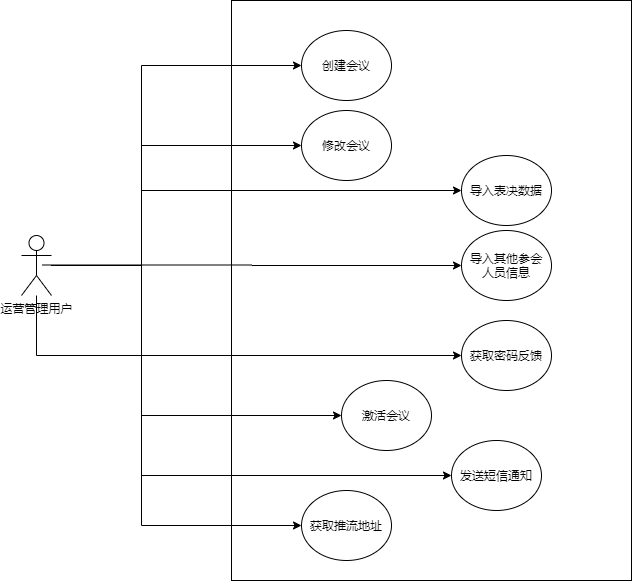
\includegraphics[height=10cm]{meetingManagement.png}
  \caption[管理模块]
    {会议系统管理模块需求用例图}
 \label{fig:meetingManagement}
\end{figure}

\subsubsection{创建和修改会议}
原系统会议模块创建和修改会议分为三步,填写会议基本信息、填写议题相关信息、导入议题表决信息。导入议题表决信息显然和创建会议属于不同功能,将导入信息作为创建会议的一环并不合理,因此将导入议题表决信息功能单独拆出。另外将创建会议拆分成两步并没有实际意义,反而增加了创建会议时出现错误的概率,因此将填写会议基本信息、填写议题相关信息合并为一步。

运营管理人员在运营平台创建和修改会议。创建和修改会议需要填写会议的基本信息(会议名称和会议召开日期为必填项)、会议的议程信息(包括需表决和无需表决议程)、议程的表决组信息,由于向 OSS 文件系统存储会议文件和议程文件时,需要会议号作为索引,因此在创建会议前需要提前向后端请求获取预约会议号。

\subsubsection{导入表决数据和其他参会人员信息}
表决数据包括表决信息(表决所在表决组、表决金额等)和表决信息对应的债权人信息。原系统会议模块导入表决数据是创建会议的第三步,表决数据仅可导入原债权申报系统中已存在的数据,若仅使用会议功能,表决数据的导入和原债权申报系统数据强绑定的设计就显得极为不合理。因此将导入表决数据和原债权申报系统数据解除绑定,改为使用 Excel 文件上传导入表决数据。点击下载 Excel 模板,填写完表决数据完整信息后,点击导入表决数据上传填好的 Excel 文件。此时,可能存在债权人未在会议平台注册的情况,表决数据若对应已存在债权人,则将表决数据划分给已存在债权人。表决数据若对应不存在债权人,则先创建对应债权人,再将表决数据划给创建的债权人。

会议除相关管理人和债权人外,还存在其他参会人员(仅可观看会议)。其他参会人员不可自行注册,仅可通过运营人员在运营平台通过上传 Excel 文件导入,目的是为了防止会议无关人员参与会议。

\subsubsection{发送短信通知}
与原系统会议模块相比,增加了短信通知功能。运营平台管理员可以向所有会议相关人员发送短信通知。选定模板和发送范围后,可以向指定范围发送会议相关信息。

\subsection{会议系统主模块}

原系统会议模块用户分为两类。一是管理人用户,二是债权人用户。若存在仅可观看会议的其他类型参会人员,需注册为债权人用户,不赋予表决数据,即可满足只能观看的需求。这种做法不符合规范,因此新增游客用户类型,仅提供观看会议的权限。

会议系统主模块负责会议的核心功能。视频表决会议系统的用户分为三类。一是管理人用户,二是债权人用户,三是游客用户(即其他参会人员)。管理人用户具有开启表决、结束表决、查看表决详情、查看参会详情、设定结束日期、查看会议详情、查看会议列表、观看视频直播、实时聊天的功能。债权人用户具有签到、补签、投票表决、实时聊天、查看会议列表、查看会议详情、观看视频直播的功能。游客用户具有查看会议列表、查看会议详情、观看视频直播的功能。会议系统主模块的具体功能需求如图~\ref{fig:meetingMain} 所示。

会议系统主模块功能根据是否有实时性要求又分为实时模块和非实时模块。实时模块包括实时聊天功能和投票表决功能。

\begin{figure}[!htp]
  \centering
  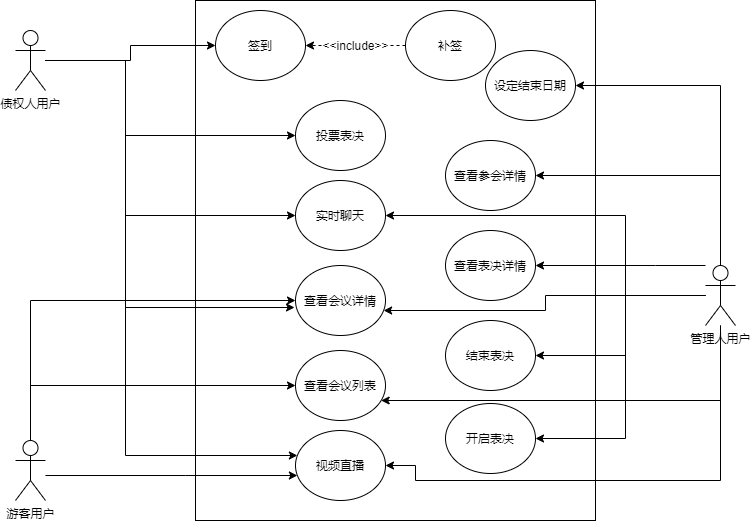
\includegraphics[width=12cm]{meetingMain.png}
  \caption[主模块]
    {会议系统主模块需求用例图}
 \label{fig:meetingMain}
\end{figure}

\subsubsection{开启和结束表决}
原系统会议模块的表决开启和结束由创建会议时设定的开启日期和结束日期决定,由于实际需求中,会议的表决开启和结束有时需要管理人进行控制,因此管理人用户增加了开启和结束表决的功能。

\subsubsection{查看参会详情和表决详情}
原系统会议模块仅有参看表决详情功能。在实际的会议中,管理人有时需要向法院报告会议参会情况,因此管理人用户增加了查看表决详情的功能。

\subsubsection{签到和补签}
原系统会议模块中,债权人参加会议功能在任何时间都可以使用,即时会议已经结束,债权人仍可点击参会,这与常理不符。现在改为债权人在会议开始到会议结束之间第一次进入会议时,会主动弹出签到框,提醒债权人签到参会,并提供补签功能,签到成功后才可进行投票表决。

\section{架构设计}
在破产领域中,债权人会议和表决的意义十分重大,决定着一个破产项目的走向。在一次实际的债权人会议中,债权人的数量级平均为千人级别,有些会议的债权人数量甚至可以达到上万人。债权人会议的一项重要工作是进行表决。在实际的会议中,表决可能在较短的时间内进行,因此会导致在短时间内出现大量请求。当同时有多个会议进行时,短时间激增的请求会给服务器带来极大的压力,因此需要针对性的设计架构应对此问题。

\subsection{现有架构及问题}

\subsubsection{现有架构}
\begin{figure}[!htp]
  \centering
  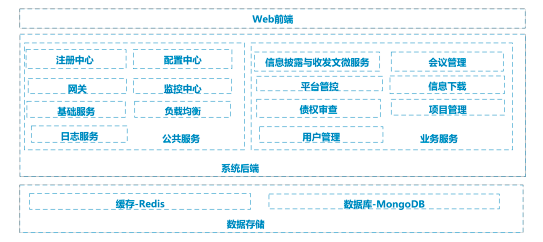
\includegraphics[width=12cm]{oldMeeting_1.png}
  \caption[原微服务]
    {原系统微服务架构图\cite{Wang2021}}
 \label{fig:oldMeeting_1}
\end{figure}

原系统采用微服务架构的原因一是原系统已具有比较完整
的服务治理管理体系,采用微服务架构将节省部署运维和降低系统升级的工作难度。这样
就能充分复用原系统的实现,减少开发系统,升级系统的成本。二是可以满足系统可
扩展性的要求。当需要对系统持续升级与优化时,可以直接设计其他微服务加入到微
服务治理体系中以满足用户不断扩展的需求。具体架构如图~\ref{fig:oldMeeting_1}\cite{Wang2021} 所示。根据微服务架构设计的高内聚低耦合的原则,原系统将会议管理整体划分为一个微服务,所有会议相关的功能全部集中放在会议管理微服务中。

在原系统的设计中,当用户数上升时,可以为各个微服
务起多个实例同时服务来满足用户并发数,可以在不改变软件架构的基础上通
过增加硬件资源来提高服务质量。

\begin{figure}[!htp]
  \centering
  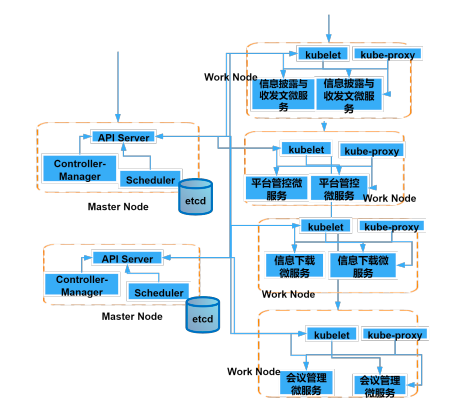
\includegraphics[height=8cm]{oldMeeting_2.png}
  \caption[原物理架构]
    {原系统物理架构图\cite{Wang2021}}
 \label{fig:oldMeeting_2}
\end{figure}

原系统是在 k8s 集群上进行部署的,系统采用图~\ref{fig:oldMeeting_2}
的物理架构。系统用户可以直接通过浏览器访问系统。而用户的请求都将到达 K8s 集群中
的 Mater Node,由 Master Node 结点进行处理。Mater Node 结点是整个集群的管理结点,该
结点会根据请求的特性命令 Work Node 结点进行作业工作。另外,一个服务往往运行成多个实例以增加系统的容错性。


\nocite{Wang2021}
\subsubsection{存在问题}

在网络债权人会议中,保证实时性非常重要。在原系统的实现中,会议管理微服务实现为 SpringBoot 后端,在会议管理微服务中通过 WebSocket 实现实时聊天,通过轮询实现管理人查询数据的实时更新。

首先,假设系统需要能同时处理 1 万场会议,每个会议债权人数量为 1万人,仅仅实时聊天的长链接数量就达到了1亿级别。SpringBoot 项目的默认启动容器是 Tomcat,而 Tomcat 默认支持的连接数量为 1 万,这个数量级远远低于要求。如果将 WebSocket 实现在 SpringBoot 项目中,需要调大 Tomcat 的连接数量或者更换启动容器,即使更换启动容器将连接数量扩大至百万级,按照原系统设计为会议管理微服务起多个实例同时服务来满足并发数需要启动接近1百个实例,这仅仅是为了满足保持实时聊天的长连接数量。

其次,通过轮询方式实现管理人端查看数据的实时更新,会给服务器带来较大的压力,且比较浪费资源,债权人侧投票表决和管理人侧数据实时刷新也应当通过 WebScoket 实现。

我们发现在会议系统中,需要通过 WebScoket 实现的功能和其余功能是独立的,并且在现有设计下为了保证 WebScoket 的长连接数量会给服务器带极大压力和资源浪费,因此考虑将 WebSocket 相关功能拆出实现为独立的微服务。

\subsection{架构设计}
将原本的会议管理微服务拆分为会议管理微服务(除去实时功能)、实时表决微服务和实时聊天微服务。新的会议管理微服务仅包含基础功能(创建会议等),与原本实现差别不大。会议开始前和会议结束后的表决数据查询通过会议管理微服务,而在会议进行中时,表决数据查询通过实时微服务进行,后面主要介绍实时微服务架构设计。由于进行表决时,实时请求数量激增,为了防止 SpringBoot 后端压力过大,使用 Kafka 集群进行流量削峰。

\begin{figure}[!htp]
  \centering
  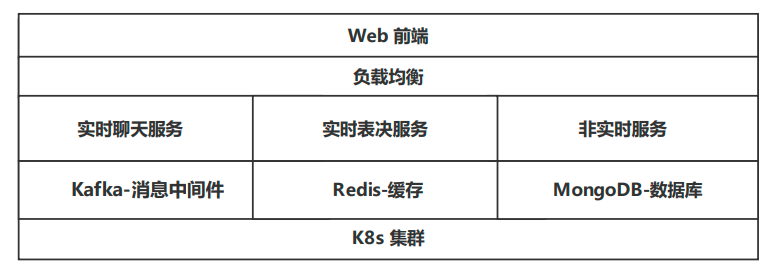
\includegraphics[width=12cm]{cluster.png}
  \caption[实时微服务架构]
    {WebScoket 服务架构图}
 \label{fig:cluster}
\end{figure}

针对系统的某个实时微服务,如表决服务、聊天服务,所有用户均使用同一套服务架构。
该服务架构一定包括无状态的 WebSocket 服务实例集群,以及独立的有状态 Redis 集群。Redis 集群是实例的状态中心,存储实例的所有状态数据。实时服务将数据成功写入 Redis 集群后生产一条消息发往 Kafka 集群,SpringBoot后端集群成功消费消息后,将数据写回至缓存 Redis 集群,Redis 集群通过 Write Back 策略将数据写回 Mongo 集群。


\section{本章小结}
本章首先对视频表决会议系统的需求进行了分析,将会议系统分为了管理模块和主模块两部分,分别画出了会议系统的需求用例图,并对新系统和原系统在功能需求上的差异做出了对比并说明了原因。在需求分析完毕之后,本章先介绍了原系统的架构设计,说明了原先架构存在的问题并针对现有会议功能需求,给出了针对性的架构设计。
\chapter{系统后端设计与实现}
本章节主要介绍系统后端针对不同业务做出的设计,包括数据结构设计和算法设计和实现。

本会议系统的后端涉及到的角色有四种,一是运营人员,二是管理人,三是债权人,四是其他参会人员。涉及到的主要功能有会议基本信息的增删改查、会议的数据导入(包括表决数据导入和其他参会人员信息导入)、直播服务、实时聊天室、实时表决服务等。根据是否和实时性相关将本系统的后端主要分为两个部分,一是非实时服务部分的后端,实现为 SpringBoot 后端; 二是实时服务部分的后端,实现为 WebSocket 后端,后文将对两部分分开进行介绍。

实时服务后端所用到的数据结构全部来自于 SpringBoot 后端,因此数据库设计仅展示 SpringBoot 后端的数据库设计。

\section{数据库设计}
如图~\ref{fig:meetingER}所示,整个系统的数据实体被划分为 Meeting, Schedule,
Group, Ticket, MeetingCreditor, ChatRoom 这 6 种类型的实体以满足需求。其中 Meeting 表示会议, Schedule 表示议程, Group 表示表决组, Ticket 表示选票, ChatRoom 表示会议聊天室。

\begin{figure}[!htp]
    \centering
    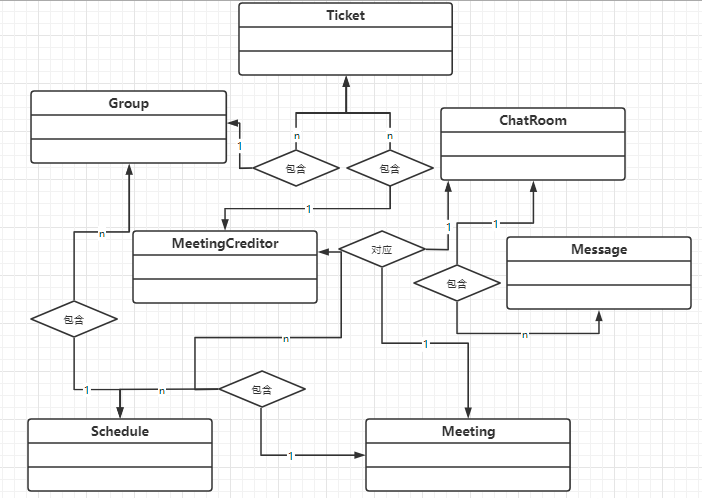
\includegraphics[height=10cm]{meetingER.png}
    \caption{会议系统数据库 ER 图}
    \label{fig:meetingER}
  \end{figure}

本系统使用 Meeting、Schedule、Group 数据实体满足会议信息管理的需求,他们分别表示了会议的基本信息,会议议程信息,议程表决组信息。Meeting 包含了会议的会议名称、创建时间、案件编号以及对应的聊天室 id 等基础信息,Schedule 包含了议程的名称,对应的会议 id ,议程的类型等信息, Group 包含了表决组名称,对应的议程 id 等信息。MeetingCreditor 满足了会议债权人管理的需求,保存着代理人代理的会议债权人的信息。Ticket 满足了投票表决的需求,它包含了选票对应的会议债权人的 id ,对应的表决组 id ,对应的表决金额以及选票的赞成或反对等信息。 ChatRoom 和 Message 满足了实时聊天的需求,其中 Message 包含了所属聊天室 id ,消息内容,发送时间和接收人(接收者的 userId,为空 null 或 [] 则为广播群发)等信息,聊天室包含聊天室的开启状态和禁用用户列表等信息。

\section{非实时后端设计与实现}
非实时后端包含了所有非实时性的功能,主要包括会议基本信息的增删改查、会议的数据导入(包括表决数据导入和其他参会人员信息导入)、其他参会人员登录及直播服务。


\subsection{会议基本信息管理的增删改查}
\subsubsection{创建和修改会议}
在原系统中议程被称为议题,下面统称议程。原系统会议模块创建和修改会议分为三步,分别是填写会议基本信息、填写议程相关信息、导入议程表决信息,只有三步全部完成会议才能创建成功,否则为暂存状态。原本的设计存在一些问题,一是会议创建分为三步过于累赘,导入议程表决信息并不属于创建会议的工作。二是会议和表决强绑定,仅含有无表决议程的会议无法通过导入议程表决信息这一步。

基于以上问题,对创建和修改会议进行了调整。一是将填写会议基本信息和填写议程相关信息合并为一步。在实际实现的时候发现创建会议时,在创建会议请求发送以前,就需要获取会议 id 用于存储会议文件和议程文件至 OSS 文件系统对应会议 id 目录下,因此在创建会议前需要先获取会议 id 。本系统会议的 id 号由 redis 数据库存储的对应 id 控制,因此在创建会议前,先向 redis 预约一个会议 id, 在创建会议时将对应会议文件和议程文件存至 OSS文件系统对应目录下,由于从 redis 中获取 id 后,设置了 id 自增,因此会议 id 号预约唯一。并且由于创建会议时,有多个实体需要存至Mongo数据库,因此实现方法时添加了SpringBoot 的事务性注解,一旦创建会议失败,回滚所有数据库操作。二是将导入议程表决信息从创建修改会议中拆出,仅含有无表决议程的会议也可以正常创建会议,而导入议程表决信息仅有含有需表决议程且导入标记为 false 的会议需要进行,通过这样的设计,仅无表决议程的会议可以正常完成流程。

\subsubsection{删除会议}
原系统会议模块中,删除会议为直接从数据库中删除对应会议全部数据,由于需要规避误删及恶意删除的情况以及需要提供删除恢复的功能,直接从数据库中删除数据的方式不可取,本系统删除操作全部改为采用逻辑删除,对应实体添加 deleted 字段用以表示对应数据是否被删除,为 true 则表示该数据已被删除。

\subsubsection{查询会议}
和原系统会议模块相比,查询会议功能主要有两个重要的变化。一是由于新系统删除操作全部改为逻辑删除,因此在查询时需要根据 deleted 字段进行筛选,获取未被删除的数据。二是原系统会议模块会议的状态是通过获取会议列表事件进行驱动的,在每次获取会议列表时,会对获取到的会议进行一次处理,根据会议召开时间和当前服务器时间的对比重新更新会议状态。在每次获取会议列表时,都会进行这样的操作,假设有 1000 个人拥有1个同样的会议,他们每个人获取一次会议列表,这个会议的状态都会被更新1000遍,即这个会议会被重新存储1000次,如果短时间内大量的人获取会议列表,且每个人会议列表包含的会议数量都不少的情况下,服务器的资源可能很快就被耗尽,这是不可取的。会议的状态仅仅是前端展示的一个维度,不需要存入数据库,只要在获取会议列表时通过会议召开时间和当前服务器时间的对比设置返回给前端的会议状态字段即可。

\subsection{会议系统的数据导入}
会议系统的数据导入分为两个部分,一是表决数据导入,二是其他参会人员信息导入。

原系统的表决数据导入为直接从债权审查模块拉取审查数据,如果用户仅仅使用会议系统而不使用债权审查,会议就无法获取相关数据,会议无法正常进行。这种情况下,会议系统和债权审查系统就变成了强绑定关系,而这是不合理的。因此需要新增额外的导入手段,本系统使用的导入方式是Excel模板导入的方式。用户先从前端点击下载表决数据导入的模板,在填入对应信息后上传表决数据表格,SpringBoot 后端通过逐条读取表决数据表格,导入相关表决信息,若代理人或会议债权人不存在,还需要通过表中信息自动创建代理人和会议债权人,多次导入时,如果对应选票数据存在则进行复用,表中有但数据库中无对应数据的进行创建操作,剩余的上一次导入数据全部逻辑删除,所有存储操作在导入模板数据全部读取完成后进行,若读取发现模板存在错误,则此次导入数据不存回数据库,并将错误信息通过Excel表格返回给用户。表决信息模板如表~\ref{fig:meetingImport}所示。

\begin{table}[h!]
    \begin{center}
      \caption{表决信息导入模板}
      \label{fig:meetingImport}
      \begin{tabular}{|c|c|c|c|c|c|}
        \textbf{债权人名称} & \textbf{编号} & \textbf{债权所在表决组} & \textbf{表决金额} & \textbf{参会人姓名} & \textbf{参会人手机号}
      \end{tabular}
    \end{center}
  \end{table}

本系统由于除开参与会议管理的管理人和行使表决权利的债权人外,还有一些其他的参会人员,如法官、无表决权债权人等,只参观会议的进行,不参与其他操作。为了更好地区分,额外设置了其他参会人员,其他参会人员的信息在表决信息导入后,也通过 Excel 表格进行导入,导入方式同表决信息导入,其他参会人员仅参观会议,实际上只在会议进行期间有效,因此其他参会人员信息存入 Redis,无需持久化到 Mongo 数据库,一旦会议结束即可删除。导入其他参会人员信息模板如表~\ref{fig:otherUserImport}所示。

\begin{table}[h!]
    \begin{center}
      \caption{其他参会人员信息导入模板}
      \label{fig:otherUserImport}
      \begin{tabular}{|c|c|c|}
       \textbf{参会人姓名} & \textbf{参会人手机号} & \textbf{参会人类型}
      \end{tabular}
    \end{center}
  \end{table}

在实现了导入后,由于导入模板中存在的新的代理人和会议债权人为系统自动创建,密码也由系统自动创建,而 user 后端的数据加密方式为非对称加密,无法通过数据库中存储的加密 password 字段反向获取明文的密码,因此需要提供自动生成密码的反馈给用户,由于导入可以重复进行,若将密码生成放在导入时,可能会重复进行多次生成密码,这样变相产生浪费。因此改为信息导入都成功后,点击生成密码则会调用生成密码接口自动为对新创建的代理人和会议债权人创建密码,并将生成的密码导出至 Excel 返回并将密码在 OSS文件系统中备份,如果需要再次获取密码,则点击生成密码反馈,直接向 OSS 文件系统请求获取生成密码的 Excel 备份文件。生成密码反馈 Excel 如表~\ref{fig:passwordReturn}所示。

\begin{table}[h!]
    \begin{center}
      \caption{密码反馈模板}
      \label{fig:passwordReturn}
      \begin{tabular}{|c|c|c|c|c|}
       \textbf{用户名称} & \textbf{手机号(登录账号)} & \textbf{密码} & \textbf{用户类型} & \textbf{代理债权人名单}
      \end{tabular}
    \end{center}
  \end{table}

  \subsection{其他参会人员登录}
  前面提到其他参会人员实际只在会议召开期间有效,且信息不会持久化到 Mongo 数据库,如果使用密码登录,显得比较累赘,因此考虑使用其他登录方式。首先考虑的是使用游客链接登录的方式,直接向其他参会人员发送可以参会的游客链接,点击即可入会参会。管理人反馈使用链接登录和使用账号密码登录对于管理人通知来说是两种参会方式,要减轻管理人的负担,应该让代理人可以通过一致、统一的方式登录,方便管理人沟通,且使用管理人认为链接可以随意转发,会议安全性无法保证。

  游客登录方案不可行,参考目前各系统通用的登录方式后决定使用手机号验证码登录的方式,既可以保证安全性,又不需存储其他参会人员的密码,方便快捷。其他参会人员使用验证码登录时,在 sms 后端生成验证码并通过阿里云短信服务接口向对应手机号发送短信,获得成功反馈后将验证码存至 Redis, 其他参会人员填写发送登录验证请求后,向Redis获取验证码进行对比,若验证码仍在15分钟有效期内,且登录验证码和Redis所存验证码相符合,则登录成功并将 Redis中存储的对应验证码清除。

  \subsection{直播服务}

  \begin{figure}[!htp]
    \centering
    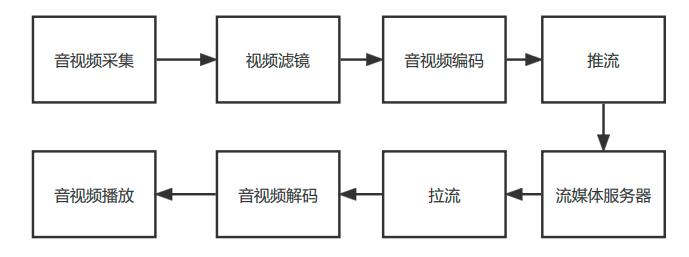
\includegraphics[height=6cm]{live.png}
    \caption{直播服务流程示意图}
    \label{fig:live}
  \end{figure}

  如图~\ref{fig:live}所示,目前直播服务的流程都是先进行音视频采集,然后进行视频的滤镜转换,转换后进行音视频编码,将编码好的音视频推流至流媒体服务器,播放端向流媒体服务器进行拉流,然后对拉取的流进行音视频解码,最后播放。目前本系统直播服务音视频采集、视频滤镜、音视频编码、推流的方式是通过摄像机采集音视频、控制滤镜,音视频编码和推流通过美菲特 M3803 编码器编码并推流。
  流媒体服务器使用的是阿里云直播服务,前端向后端发送请求,后端通过 API 向阿里云直播服务获取拉流地址。

  在使用过程中发现,单一推拉流不够稳定,在长时间的直播中可能出现断线的情况,这对视频表决会议来讲是不可接受的,为了解决这个问题,本系统采取了多路推流的方式,同时将一个直播流向多个推流地址进行推流,当一个推流地址出现问题时,可以通过切换线路保证直播服务的质量。

  \section{实时后端设计与实现}
  实时后端包含了所以具有实时性的服务,包括聊天室服务和实时表决服务。WebSocket后端使用Golang实现。

  \subsection{WebSocket 业务通信协议}
  在系统的实际业务中,WebSocket 消息传输为双向的。任一端都是 client 和 server。
无论 client 或 server,WebSocket 的所有消息入口只有一个。消息又只发向数个业务中的一个。
并且,根据网络 e2e 通信原则,“at least once” 的请求在业务层必须作出显式响应。
因此,本节将给出所有 WebSocket 业务通信协议的规范和定义,如图~\ref{fig:wsxy}所示。

\begin{figure}[!htp]
    \centering
    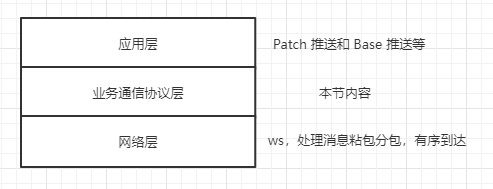
\includegraphics[height=6cm]{wsxy.png}
    \caption{WebSocket 业务通信协议示意图}
    \label{fig:wsxy}
  \end{figure}

  \subsubsection{消息类型}
  Client 与 server 间通信只接受 JSON 格式的 “消息”。
  消息分为多种类型,一种是请求型,一种是相应型,如图~\ref{fig:messageType}所示。
  
  \begin{figure}[!htp]
    \centering
    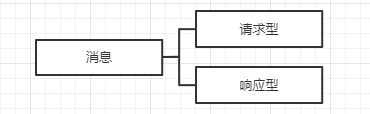
\includegraphics[height=2.5cm]{message.png}
    \caption{消息类型}
    \label{fig:messageType}
  \end{figure}

  请求型消息,可由 client 或 server 发起,向对方请求内容或推送内容,格式如下方代码展示。
  {\setmainfont{Courier New Bold}
\begin{lstlisting}
    // 请求型消息
    {
        "t": "req",    // type
        "i": string,   // 消息 id。为随机数。如果 id 为 0,则代表该请求无需对方响应
        "h": string,   // handler。即 server 对应处理方法名
        "d": object    // data
    }
 \end{lstlisting}}

 响应型消息,对请求型消息的回复,格式如下方代码展示。
 {\setmainfont{Courier New Bold}
 \begin{lstlisting}
    // 响应型消息
    {
        "t": "res",    // type
        "i": string,   // 所响应的请求型消息的 id
        "s": number,   // HTTP 状态码,与 Restful 接口对齐,即可复用 Restful 接口的代码
        "d": object    // data
    }
  \end{lstlisting}}

  \subsubsection{消息处理}
  WebSocket 连接的每一进程都同为 server 和 client,且每一进程的所有消息同享一个入口。
对于每一个 WebSocket 进程:

\quad{}1. 作为 server 时会注册一系列方法,用于处理 d 字段的数据。

\quad{}2. 作为 client 时会发送一系列消息,并等待响应结果返回给上层。

两进程的通信如图~\ref{fig:wsConnect}所示,蓝色 server 和 client 为同一进程,而黄色为另一进程,它们互相通信。
\begin{figure}[!htp]
    \centering
    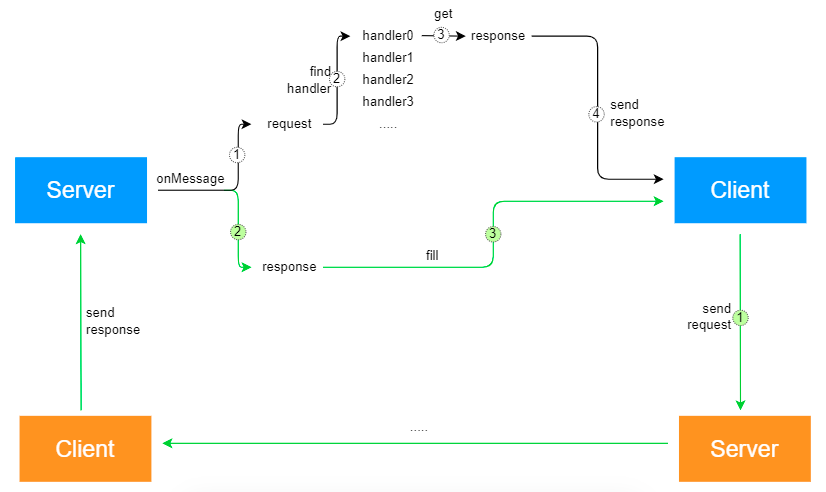
\includegraphics[height=7.5cm]{wsConnect.png}
    \caption{消息处理}
    \label{fig:wsConnect}
  \end{figure}

白色数字标识 server 服务流程:

\quad{}1. 服务端收到信息,检测 t 字段为 req,即为请求;

\quad{}2. 根据信息 h 字段,寻找对应的 handler 以处理 d 字段中的数据;

\quad{}3. Handler 返回请求结果。注意,若未找到 handler,则用默认 handler,返回错误信息;

\quad{}4. 使用本实例的 client,向黄色进程发送返回结果,流程结束;

绿色数字标识 client 需要 server 响应的请求流程:

\quad{}1. client 发送请求消息。上下文进入等待状态。若超时后则 abort(非幂等请求除外);

\quad{}2. 进程执行上文 server 相同流程。流程结束后,本进程收到对应请求的响应消息;

\quad{}3. 将响应消息填充向处于等待状态中的请求上下文,结束等待。

对于不需要 server 响应的 client,其发送的请求中 i 字段为 0。

\subsubsection{Golang 端}
Golang 端中的一份 WebSocket 连接分为两个协程处理,分别进行读操作和写操作的同步。
一个连接所涉及的所有协程均采用 context 进行结束。

Golang 端内部有一个 pendings map,专门用于等待用户的响应型请求。
map 的 key 是请求 id,值是响应型消息的指针的 chan(信道)。

如果要写入请求型消息,对于要用户响应的消息,随机生成一个请求 id,向 pendings map 中注册一个 chan(信道),在该 chan(信道) 上进行等待。
对于不需要用户响应的请求型消息,保持请求 id 为 0,跳过 pendings map 流程,直接写入即可返回。

如果要写入响应型消息,直接写入即可。

对于收到的请求型消息,根据请求型消息的 h 内容,调用程序内不同的 handler。handler 处理后,生成对应的响应型消息,发送给写协程返还给用户。

对于收到的响应型消息,根据其消息 id,找到 pendings map 中正在等待的 chan(信道),向其中写入该消息,让等待消息的协程结束等待。

\subsubsection{JavaScript 端}
JavaScript 端由于浏览器为单线程执行,因此无需关心同步异步的问题。

JavaScript 端内部有两个 map,一个存所有的 handler,一个存所有在等待的 Promise,kv 结构与 Golang 端类似。

如果要写入请求型消息,如果需要返回,则创建一个随机数作为请求 id,再创建一个 Promise 放入等待 map 中,并返回这个 Promise。
如果不需要用户响应的请求型消息,则保持请求 id 为 0,跳过 Promise 放入等待 map 等过程,直接返回即可。

如果要写入响应型消息,直接写入连接即可。

对于收到的请求型消息,根据请求型消息的 h 内容,调用 handler map 中不同的 handler,待其处理后生成对应的响应型消息,直接写入连接中。

对于收到的响应型消息,在等待 map 中找到对应的 Promise,根据消息的 s 进行 resolve 或 reject。

JavaScript 端代码完全用 class 实现,与 React 交互时会产生函数作为状态无法正确更新的问题,后续需换用自定义 hooks 实现。

\subsection{实时聊天室服务}
聊天室服务用于支持表决会议在线聊天,考虑到聊天室支持私聊,因此,每个用户在聊天室中的可见内容不同,即它们的 View 互不相同。
若聊天室同时服务数千人,则服务内部有数千份 View。
如果对每个人进行完整的 Base 推送,根据性能测试结果不能达到预期。

开销来源于重复 marshal,每个用户的 View 中有大量相同数据。
实时聊天室不同于表决服务,每位用户在聊天室中所见的消息是增量的,每份 View 的内容都是增量的,并且每个人的 View 又很可能重叠。这会导致大量计算开销。

\subsubsection{优化设计}
考虑到聊天室数据的本质是一个只读的,持续增长的消息序列并且聊天室并不存在聚合数据,只有同源数据,不需要定时的重新聚合计算任务。
因此,对连接上同一个聊天室的每个用户而言,可以认为所有人共享一个 View,其内部包括所有人发送的所有信息,只不过在 Base 请求时每个人可见的内容不同。

根据这种考虑,聊天室无需存储每个用户的数千个 View,只需存储一个 View,即一个持续增长的数组。
在这个设想下,系统内每条 Message 都有了先后顺序,它们在数组中的索引有序且唯一。
Message 的先后顺序能让聊天室快速构造 Base 推送。
只有用户知晓其接受到了多少 Message,只需定时告知聊天室,即可反推出所缺失的 Message。
用户请求包括两个字段,自己的最新 Message 索引号,以及自己的已知缺失 Message 数组。
聊天室的响应即 Base,包括用户的已知缺失的,以及用户最新至聊天室最新之间的 Message,如图~\ref{fig:wsChatRoom}所示。
\begin{figure}[!htp]
    \centering
    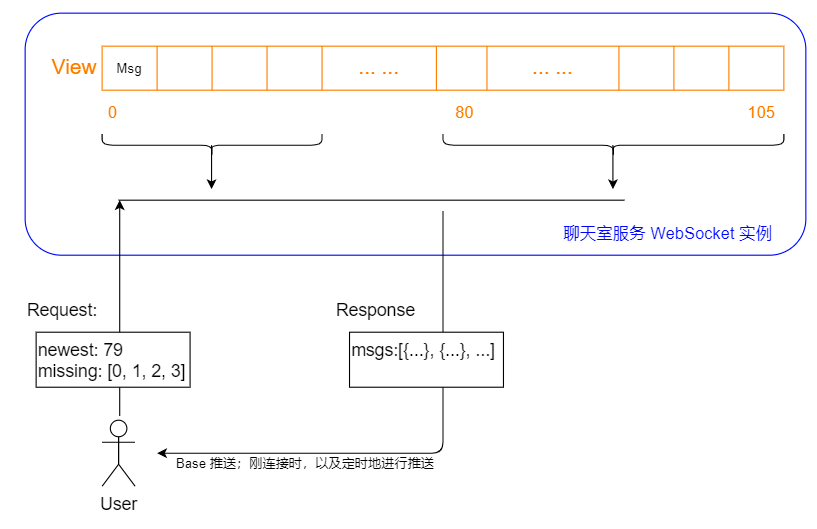
\includegraphics[height=7.5cm]{wsChatRoom.png}
    \caption{聊天室优化方案}
    \label{fig:wsChatRoom}
  \end{figure}

  \subsubsection{部分实现}
  1. Handshake:会话握手请求

  仅限用户发向实例。
  必须在用户握手成功,建立起会话数据后,服务端才会处理用户发来的请求。

  如果该用户已有会话,则强制原有会话下线。

  {\setmainfont{Courier New Bold}
  \begin{lstlisting}
    // 参数:
    {
        "userId": number,
        "chatroomId": number,
        "userType": string, // 用户类型,只接受 PRACTITIONER 和 CREDITOR
        "userName": string
    }
    // 响应:
    null
   \end{lstlisting}}

   2. GenerateBase:生成 Base 推送

   仅限用户发向实例。
   遍历当前 View,返回该用户可见的消息。

   {\setmainfont{Courier New Bold}
   \begin{lstlisting}
    // 参数:
    {
        "missingMsgIds": number[], // 用户已知的缺失的消息 index
        "newestIndex": number // 用户目前收到的最新的消息 index
    }
    // 响应:
    {
        "bannedUsers": number[], // 该用户可见的当前被 ban 的用户 id 列表;管理人可见所有人,债权人只可见自己
        "messages": Message[]
    }
    \end{lstlisting}}

    3. DownloadMessages:下载聊天记录

    仅限用户发向实例。仅管理人可用,下载整个 View 内的所有内容,无论其对该管理人是否可见。
 
    {\setmainfont{Courier New Bold}
    \begin{lstlisting}
        // 参数
        null
        // 响应
        Message[]
     \end{lstlisting}}

     4. NewMessage:发送新消息

     仅限用户发向实例。
     仅用户未被 ban 时,且聊天室未关闭时可用。
     在 View 数组放置一个空消息,放锁,将消息存入 Reids。
     成功后,该消息会存入 View 数组中对应的空消息处,并引发一次 patch 推送。
  
     {\setmainfont{Courier New Bold}
     \begin{lstlisting}
        // 参数
        Message
        // 响应
        {
            "index": number // 所发送的消息在 View 的消息数组中的 index
        }
      \end{lstlisting}}

      5. Ban:封禁 / 解禁用户

      仅限用户发向实例。
仅聊天室未关闭时可用。
仅管理人可用,且不可封禁管理人。
   
      {\setmainfont{Courier New Bold}
      \begin{lstlisting}
        // 参数
        {
            "userId": number,
            "ban": bool // 指明该用户是否被 ban
        }
        // 响应
        null
       \end{lstlisting}}

       6. ForceOffline:强制用户下线

       仅限实例发向用户。
       如果用户建立会话时,已有该用户的会话,则实例会发送给被顶替用户下述内容,并在最多两秒后关闭连接。
   
      {\setmainfont{Courier New Bold}
      \begin{lstlisting}
        // 参数
        {
            "time": number, // 异地登录者的登录时间
            "ip": string // 异地登录者的登录 IP
        }
        // 响应:无需响应
       \end{lstlisting}}

       7. patchMessage:用户接受消息推送

       仅限实例发向用户。
       在用户发送新消息,并成功保存后,对应的消息会 Patch 推送给发送者和接受者。
   
      {\setmainfont{Courier New Bold}
      \begin{lstlisting}
        // 参数
        Message
        // 响应:无需响应
       \end{lstlisting}}

       8. patchBan:用户接受 ban 推送

       仅限实例发向用户。
在用户的 ban 状态产生变化,并成功保存后,对应的消息会 Patch 推送给被 ban 人和全体管理人。
   
      {\setmainfont{Courier New Bold}
      \begin{lstlisting}
        // 参数
        {
            "userId": number,
            "ban": bool // 指明该用户是否被 ban
        }
       \end{lstlisting}}

  \subsubsection{交互设计}
  考虑到所有用户共享一个 View,其包括所有用户的聊天发言和封禁状态,因此每个用户在前端也维护类似这样的数据结构。具体地,前端维护:

  \quad{}1. messages 数组

  \quad{}2. bannedUsers 数组

对于一个用户来说,其不清楚不可见的信息是由于网络延迟未收到还是由于自己不可见。

对于自己不可见的 message,其 messages 数组对应 index 处为 null,即 JavaScript 语义中的 “有数据但为空”。

对于不确定是不是自己不可见,且又未收到的数据,其 messages 数组对应 index 处为 undefined,即 JavaScript 语义中的 ”不知道“。
对于每个 undefined 的数据,前端会在一定时间内发送 generateBase 请求向后端确认,到底是不是自己不可见,如果不是则返回相应数据。

对于债权人,这样的定时任务为 120s,因为单个债权人看不到其他债权人的发言,因此聊天室内消息不多,服务端向该用户的网络拥塞可能性低。

对于管理人,这样的定时任务为 10s,因为管理人几乎可以看见所有聊天内容,因此聊天室内的消息很多,必须得确保内部的消息的正确性和及时性。

\subsection{实时表决服务}

\subsubsection{实时表决服务流程设计}
以管理人为例,实时表决服务流程如图~\ref{fig:wsbjlc}所示。

\begin{figure}[!htp]
    \centering
    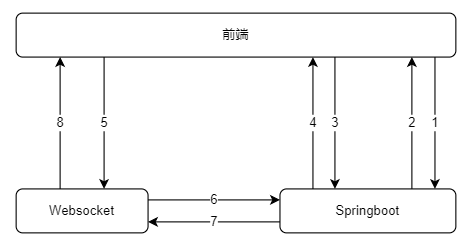
\includegraphics[height=6cm]{wsbjlc.png}
    \caption{WebSocket 表决服务流程示意图}
    \label{fig:wsbjlc}
  \end{figure}

  \quad{}1. 管理人进入会议界面,前端向 SpringBoot 后端发送请求;

  \quad{}2. 后端返回统计数据给前端,前端收到请求后将数据在前端渲染,生成视图,前端接收到数据后需要将数据持久化到客户端上,从而减少后端每次计算全量数据的压力。为了明确前端数据是否需要被更新,后端数据应当给统计数据维护一个类似版本号的字段,若发现版本号变更,则更新数据,重新从 springboot 拉取一遍全量数据;

  \quad{}3. 前端询问会议是否已结束;

  \quad{}4. Springboot 返回会议结束标识,若:

  \quad{}\quad{}a. 会议已结束,该流程结束;
  
  \quad{}\quad{}b. 会议未结束,进入第 5 步;
  
  \quad{}5. 会议未结束,则管理人和后端建立 websocket 链接,等待数据推送;
  
  \quad{}6. Websocket 获取会议相关 Entity,数据不存在,向 Springboot 发起数据请求,只有 websocket 本地没有缓存全量 Entity 时才会向 springboot 返回全量的数据,其他时候直接依据内存 / Redis 返回的缓存计算结果;
  
  \quad{}7. Springboot 返回所有的 Entity,Websocket 将其缓存在 Redis 中,并缓存在内存中;
  
  \quad{}8. Websocket 根据实际情况实时推送数据到前端,前端依据 Websocket 推的数据进行更新,websocket 不会返回给前端全量的数据,而是一个数据片段,包含各个议题的表决情况、参会人数情况和被更新的数据(比如某自然人就议题 A 提了同意票)。

  \subsubsection{实时表决服务内部数据流和控制流流转}
  Websocket 会在下列场合和 Springboot 的 meeting 服务、前端(债权人端和管理人端)以及 Redis 服务进行通信:

  \quad{}1. 当 Websocket 的缓存 Redis 没有缓存会议任何数据时,Websocket 首先要和 springboot 服务通信,获取该会议下全量的 Entity,然后 websocket 将这些 Entity 全部存储到 Redis 中,同时在内存中存储一份,它们是一次会议下的 meta 数据;同时,Websocket 服务会根据得到的 Entity 数据形成一份 View 数据,View 数据表示的是各个议程的统计信息,View 数据不需要持久化到 Redis 中;
  
  \quad{}2. 对于一个债权人而言,假设此时一个债权人投了票,则投票的行为通过前端的 websocket 客户端发送到 websocket 服务,websocket 服务根据收到的投票行为首先更新 Redis 的内存,然后更新对应的内存 Entity 实例,然后将这次表决结果存储在一个 Dirty 中(Dirty 是一段时间内表决 Data 的集合),并更新 View 数据,流程如图~\ref{fig:wszqrlc}所示。

  \begin{figure}[!htp]
      \centering
      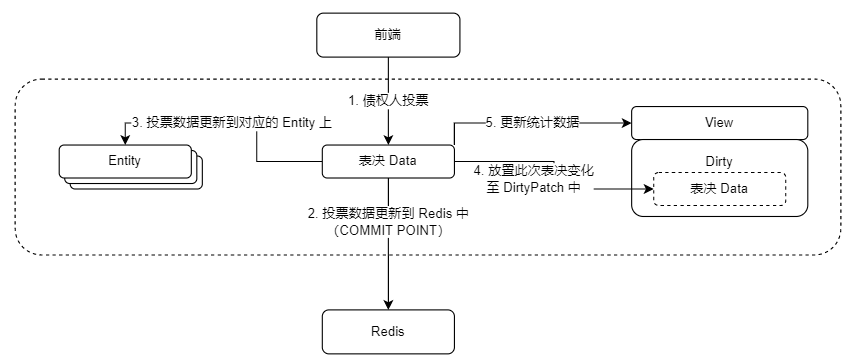
\includegraphics[height=8cm, width=12cm]{wszqrlc.png}
      \caption{债权人投票流程示意图}
      \label{fig:wszqrlc}
    \end{figure}

  \quad{}3. 对于一个管理人而言,其在一开始就已经从 Springboot 拿到了所有 Entity,因此只需要接收变化的数据和统计信息:

  \quad{}\quad{}a. 在 websocket 链接第一次创建成功时,websocket 会向管理人推一次 Base 数据,Base 数据依托于 Entity 数据生成,只记录了投了票/参了会的人员;

  \quad{}\quad{}b. 链接创建成功后,websocket 会每隔一段时间(5秒)会检查 Dirty 的数据,如果 Dirty 数据不为空,则向管理人发送 View 和 Dirty 的数据,若中间有数据发送失败,则连接断开。

% !TeX root = ../main.tex

\chapter{系统前端设计与优化}
本章节主要介绍对本系统前端相关的设计以及设计的原因和相关实现。在实现过程中有两个较为特殊的问题,一是对于管理人来说,前端已有全量的数据,计算表决结果所需的数据在前端全部都已存在,在前端进行计算的开销很少,并不需要向后端发送请求,因此将表决计算放在前端进行,为此前端设计了存储数据的前端数据库。二是由于前端不同表决类型议程的渲染逻辑区分复杂,为了解决此问题,在前端提出了一层新的抽象:表决计算精度。另外本章还介绍了前端 Redux 中的数据结构和前端实现过程中遇到的一些其他问题,下面将进行详细地介绍。

\section{前端数据库}

\subsection{设计原因}

系统前端包含一个数据库的设计来源于本系统的具体业务需求。本视频表决会议系统的目的是为了实现破产领域全流程线上办公的表决会议模块能够满足需求,对本系统来说,简化管理人的工作是核心目的。

在视频表决会议系统中,总共有三种用户,一种是管理人用户,一种是债权人用户,还有一种是其他参会人员用户。对于债权人用户和其他参会人员用户相关的功能来说,会议相关的数据请求量都很小,对于采取前端数据库方案起决定性因素的是管理人用户的功能。管理人用户有参看参会详情、查看会议详情和查看表决详情的功能,对于一个会议来说,这三个功能的数据综合起来可以囊括此会议的全量数据,而在会议进行过程中,这三个功能的数据是从 WebSocket 服务全量返回的,因此相当于在前端保存了全量的数据。

在前端拥有全量数据的情况下,可以在前端维护一个数据库,将管理人功能部分的计算交由前端进行,这样可以变相减少后端的压力。如果要将计算前后端区分完整,目前的设计下需要的代码量远远超过将计算交由前端进行,并且代码的维护会比较困难,另外前端数据库的设计是将 Redux 类比成后端数据库设计的,如果要把计算迁移到后端,可以在现有的前端计算代码上做快速迁移。因此,本系统采取了前端数据库的设计。

\subsection{存储设计}

确定了前端数据库的设计后,接下来需要考虑的是前端数据库的具体设计实现。

要实现将 Redux 作为一个数据库,首先要考虑所有实体数据的存储问题。此处以议程实体 Schedule 为例,要将所有的 Schedule 数据存入 Redux中。 如果仅仅凭借原生 JS 的方法,最容易想到的两种存储方式,一是通过数组 Array 进行存取,一种是通过对象 Object 进行存取。

首先考虑使用数组 Array 进行存储。

\subsubsection{Array 存储}

{\setmainfont{Courier New Bold}
\begin{lstlisting}
  const scheduleArr: ReduxSchedule[] = []
 \end{lstlisting}}
为了考虑使用 Array 存储是否可取,假设存在这样一种情况,有 1000 个 Schedule 发生了更新,对于用 Array 存储的 Schedule 来说,Redux 要扫描数组 1000 次,每次更新一个数据。

即如果总的议程 Schedule 数量为 N,发生更新的 Schedule 数量为 M,用 Array 存储的情况下,更新 M 条 Schedule 数据的时间复杂度是 O(N*M)。这个时间复杂度是不可接受的,因此直接用 Array 存储的方式是不可取的。

在用 Array 存储的方式不可取的情况下,考虑使用原生 JS 的另一种存储方式, 使用 Object 存储。

\subsubsection{Object 存储}

{\setmainfont{Courier New Bold}
\begin{lstlisting}
  const scheduleObj: Record<string, ReduxSchedule> = {}
 \end{lstlisting}}
为了考虑使用 Object 存储是否可取,仍然假设这样一种情况,有 1000 个 Schedule 发生了更新,在使用 Object 存储的情况下,更新每个 Schedule 的复杂度都是 O(1), 因此总的时间复杂度变成了 O(M)。

O(M) 的时间复杂度似乎能满足要求,但实际上 Object 每次的 O(1) 级别的更新都非常慢,因为 Object 的实现虽然接近哈希表,但 JS 并不期望它内部存海量数据,也不希望将 Object 当作哈希表进行使用。在存海量数据的情况下,Object 的性能会比起存储少量数据的 Object 慢几十倍,并不能完全满足系统的需求,因此直接使用 Object 存储的方式也是不可取的。


直接使用原生JS的 Array 和 Object 都不能满足需求的情况下, 考虑使用其他结构进行存储。最容易想到的就是哈希表,通过查阅资料,考虑使用在 ES6 中提出的数据结构 Map 。

\subsubsection{Map 存储}

对于在 ES6中提出的数据结构 Map ,无论存储数据的量级大小,性能的变化幅度都并不大,存取大量的数据也和存储少量数据相比性能都比较高。将 Map 和 Object 进行对比, 同等条件下 Map 比 Object 快 2.38 至 80 倍,时间复杂度保持在 O(M) 的级别, Map 的使用见下方代码展示。

{\setmainfont{Courier New Bold}
\begin{lstlisting}
  // 初始化一个 map, key 是 scheduleId, value 是 ReduxSchedule 实体
  const scheduleMap: Map<number, ReduxSchedule> = new Map()
  scheduleMap.set(12, '对应的 schedule 实体')
 \end{lstlisting}}

  使用 Map 进行存储解决了查询和更新的性能问题, 但是在使用 Map 的过程中,发现了另一个问题,满足渲染要求带来的性能损耗过大。

  React的渲染机制要求,所有数据必须是不可变的,只要状态数据 setState() 前后的数据满足:
  \begin{equation}
    (prev, curr) => (prev === curr)
  \end{equation}
  的条件,前端组件就不会触发页面渲染。

  在这种情况下,不管是使用 Array 、 Object 还是 Map ,在触发 Schedule 更新的时候,除了更新 M 条新的 Schedule 数据以外,还需要将原本的 N 条 Schedule 数据重新复制一遍,生成一个新的数据结构,而这样做的目的仅仅是为了触发 React 的渲染机制:

  \quad{}a. Array 的更新渲染时间复杂度是 O(N*M + N)


  \quad{}b. Object 的更新渲染时间复杂度是 O(M + N)


  \quad{}c. Map 的更新渲染时间复杂度是 O(M + N)

  在以上三种存储方式都不能满足需求的情况,经过进一步调研发现,使用 Immutable.JS 能够解决上述问题。

  \subsubsection{Immutable.JS}
  Immutable.JS 由 Facebook 工程师 Lee Byron 花费 3 年时间打造,与 React 同期出现,但没有被默认放到 React 工具集里(React 提供了简化的 Helper)。它内部实现了一套完整的 Persistent Data Structure,还有很多易用的数据类型。本系统选择使用了Immutable.JS 的 Map 数据结构。

  Immutable.Js 的 Map 数据结构对应于 ES6 的 Map 对象,通过使用 Map 数据结构可以解决查询和更新的性能问题。另一个需要解决的问题是由于 React 渲染机制在更新的时候需要重新复制一次数据结构所带来的损耗,而 Immutable.Js 使用的 Structural Sharing(结构共享)的方式可以解决这个问题。

Immutable 中文意义为不可变的,Immutable Data 就是一旦创建,就不能再被更改的数据。对 Immutable 对象的任何修改或添加删除操作都会返回一个新的 Immutable 对象。Immutable 实现的原理是 Persistent Data Structure(持久化数据结构),也就是使用旧数据创建新数据时,要保证旧数据同时可用且不变。同时为了避免 deepCopy 把所有节点都复制一遍带来的性能损耗,Immutable 使用了 Structural Sharing(结构共享),即如果对象树中一个节点发生变化,只修改这个节点和受它影响的父节点,其它节点则进行共享。

\begin{figure}[!htp]
    \centering
    \begin{subfigure}{1\textwidth}
      \centering
      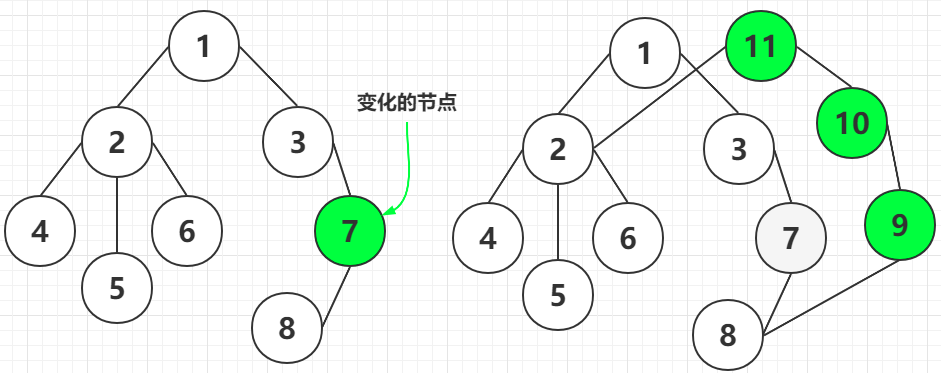
\includegraphics[height=4cm]{immutable1.png}
      \caption{}
    \end{subfigure}
    \begin{subfigure}{1\textwidth}
      \centering
      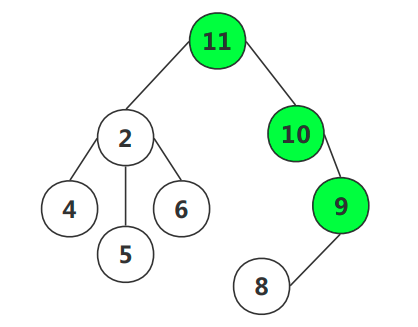
\includegraphics[height=4cm]{immutable3.png}
      \caption{}
    \end{subfigure}
    \caption{结构共享示意图}
    \label{fig:immutable}
  \end{figure}

  接下来通过一个例子介绍 Structural Sharing(结构共享),假设存在一个旧数据 oldData,它的对象树中有8个节点,如图~\ref{fig:immutable} (a)所示,现在对对象树中的节点7进行修改,这个操作将会返回一个新的 Immutable 对象。

   根据 Structural Sharing(结构共享)的原则,只修改节点7和受节点7影响的父节点,根据图~\ref{fig:immutable} (a) 可以看到受到影响的节点有节点1、节点2和节点7。对这三个节点复制一遍创建出新的节点9、节点10及节点11,节点9为节点7的复制,与原子节8相连,节点10为节点3的复制与节点7的复制节点9相连,节点11为节点1的复制,与节点1的子节点2和节点3的复制节点10相连,如图~\ref{fig:immutable} (a)所示,最后得到了一个新的Immutable 对象,如图~\ref{fig:immutable} (b)所示。

  根据前面说到的 React 渲染问题,如果使用 Map,直接更新 Map 并不能触发渲染,而使用ImmutableMap 则可以直接触发渲染,对比效果见下方代码展示。

  {\setmainfont{Courier New Bold}
  \begin{lstlisting}
    // 两种Map 的 key 都是 scheduleId, value 都是 ReduxSchedule 实体
    // ES6 Map
    const scheduleMap: Map<number, ReduxSchedule> = new Map()
    scheduleMap.set(12, '对应的 schedule 实体')
    const newMap = scheduleMap.set(14, '另一个 schedule 实体')
    console.log(scheduleMap === newMap)
    // 打印结果:true

    // ImmutableMap
    const scheduleMap: ImmutableMap<number, ReduxSchedule> = new ImmutableMap()
    scheduleMap.set(12, '对应的 schedule 实体')
    const newMap = scheduleMap.set(14, '另一个 schedule 实体')
    console.log(scheduleMap === newMap)
    // 打印结果:false
   \end{lstlisting}}

  通过使用 Immutable.js,触发渲染的性能表现如下:

  \quad{}a. Immutable.Array 的渲染时间复杂度是 O(N*M)

  \quad{}b. Immutable.Map 的渲染时间复杂度是 O(M)

  前端 Redux 通过使用 ImmutableMap,将 Redux 实现成了一个数据库,只要 Redux ImmutableMap 发生了变更,前端就触发使用该 ImmutableMap 的组件的渲染。

  在本系统设计中,使用 Immutable.Js 只是借助其Structural Sharing(结构共享)的能力减少渲染带来的损耗。而一旦将 Immutable.js 的数据结构作为业务数据,项目代码的可复用性就会变得非常差,并且无论之后进行前端做优化还是计算向后端迁移,项目代码都会变得非常难维护。在设计中ImmutableMap 只是起到像数据库一样的查询作用,所以本次设计尽量缩短了 Immutable.js 库的使用范围,仅在和表决计算相关的数据结构中使用,避免在业务逻辑用到的数据结构中使用 Immutable.js 的数据结构。这样的设计解决了前端渲染的性能损耗的问题,但是即使缩减了使用范围,仍然对本系统前端代码可维护性造成了一定影响。

  \subsection{其他问题}
  在将前端 Redux 实现为一个数据库的过程中,还有一些问题凸显了出来,这里介绍一个本系统的重要问题及解决方法或思路。

  在将前端 Redux 实现为数据库的过程中,由于各个数据之间存在有关系,例如议程 Schedule 有对应的表决组 Groups,表决Ticket 有对应的会议债权人 MeetingCreditor,这之间的对应关系的存储问题。

  目前的设计实现是实体与另一类实体的关系用外键存储,原因是只有这样才能正确触发渲染。假设在Redux数据库存储的议程实体 Schedule 中,groups 字段是一个数组,它保存了和 Schedule 相关的表决组。
  如果存的是表决组 Object ,那么表决组 Map 发生改变后,由于 groups 数组没有发生改变,用到 groups 字段的组件就无法触发渲染。
  如果存的是表决组外键,那么表决组 Map 发生改变后,由于用到 groups 数组的组件一定会用到表决组 Map,那么用到 groups 字段的组件就能正常触发渲染。

  \section{表决计算精度}
  \subsection{什么是表决计算精度}
  表决计算精度是表决前端提出的一层新的抽象,表决计算精度的定义:

  \quad{}a. 表决计算精度指的是一个议程的表决通过方式的计算精度,即指明一个议程通过与否的条件是各个表决组都得通过,还是不考虑表决组,只要议程通过即可。


  \quad{}b. 表决计算精度的概念只在需要表决的议程下出现。无需表决议程没有表决计算精度。

  表决计算精度是议程的一个字段,名称为 highPrec (boolean) 目前只在 Redux 中存在。另外表决计算精度会影响债权人、债务人表决相关的业务逻辑,进而影响前端的渲染。

  \subsection{为什么需要表决计算精度}

  首先,因为项目现在表决类型是硬编码,并不是一个变量。如果这部分的业务需求发生了变化,本系统的整个架构设计从持久层,到后端,到实时表决端,再到前端,以及接口端全部都得重修修正。一个直观的例子,由于只有重整表决需要计算到表决组级别的特殊性,本系统现有接口的命名区分为 noReorgnization (非重整表决),reorgnization (重整表决),如果新增一个议题,表决计票方式同重整表决,但命名叫新式表决,那么原本的命名 noReorgnization,reorgnization 需要改成 noReorgnizationAndNew (非重整和新式表决), reorgnizationAndNew (重整和新式表决),以及其他相关的部分全部都需要修正。如果通过表决精度来进行区分,之后的修正只需要在前端只需要加个枚举常量就可以解决问题。

  其次表决计算精度决定了前端的渲染,有了表决精度的划分,前端渲染的代码逻辑会更加清晰。例如,债权人的投票表格中,不同表决精度的议程,投票表格的行单元格合并是不同的;管理人查看表决数据统计的时候,不同表决精度的议程,表决数据统计的行单元格合并是不同的;管理人查看表决详情时,不同表决精度的议程对应的表决详情是完全不同的两张表。
  \begin{figure}[!htp]
    \centering
    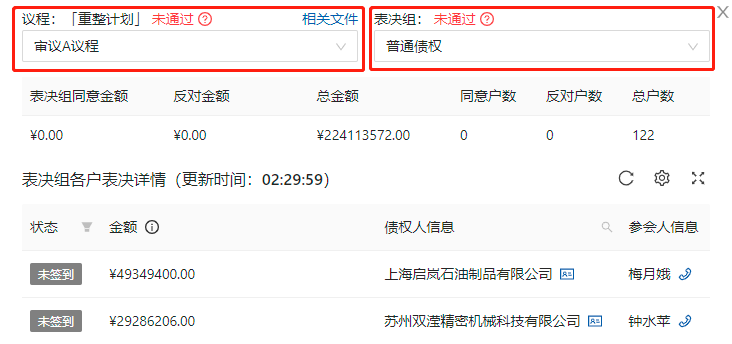
\includegraphics[height=6cm]{re.png}
    \caption{高精度议程表决详情}
    \label{fig:reo}
  \end{figure}
  \begin{figure}[!htp]
    \centering
    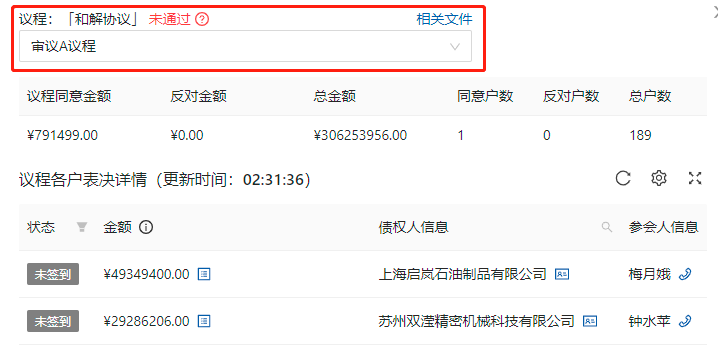
\includegraphics[height=6cm]{noRe.png}
    \caption{低精度议程表决详情}
    \label{fig:noReo}
  \end{figure}
  以管理人查看表决详情为例,从业务逻辑出发,
  高精度议程表决详情的每一行,是选中表决组下的一个表决项 Ticket,如图~\ref{fig:reo}中第一行代表债权人上海启岚石油制品有限公司在审议A议程下普通债权中的表决金额为49349400.00元。
  低精度议程表决详情的每一行,是该议程下的一个会议债权人 MeetingCreditor,如图~\ref{fig:noReo}中第一行代表债权人上海启岚石油制品有限公司在审议A议程下总共的表决金额为49349400.00元。

  总的来说,表决计算精度的提出,一是让业务代码可维护性变强了。
  二是让前端渲染逻辑更加清晰了。

  \section{Redux中的数据结构}

  在 Redux 中存储了基于 baseMeetingUser 的会议用户相关的数据结构 meetingAgent 和 meetingManager;存储了表决相关的数据结构 scheduleMap、meetingCreditorMap 和 groupMap。

  \subsection{会议用户相关的数据结构}


  \begin{figure}[!htp]
    \centering
    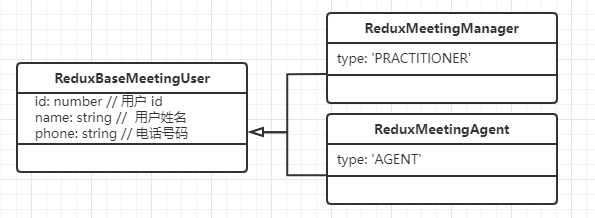
\includegraphics[height=4cm]{meetingUser.png}
    \caption{用户相关数据结构}
    \label{fig:meetingUser}
  \end{figure}

  meetingAgent 和 meetingManager 继承自 baseMeetingUser, baseMeetingUser 中包含信息用户Id,用户姓名和用户的电话号码。 meetingManager 的类型为 PRACTITIONER (管理人), meetingAgent 的类型为 AGENT (代理人),如图~\ref{fig:meetingUser}(a)。

  meetingUserState 中包含两个哈希表分别存储 meetingAgentMap 和
  meetingManagerMap 。 两个哈希表的键值对的键都是用户的ID号,值都是对应的 meetingAgent 和 meetingManager 实体。

  \subsection{表决相关的数据结构}

  scheduleType 是 Redux 中特别存储的议程类型,目的是为了方便快速地定位该议程的类型背后有关的表决信息,并由此决定前端的渲染,其中包含 name (议程类型名), description (议程类型描述), quotaPassRatio (金额通过比例), ticketPassRatio (票数通过比例), highPrecision (是否高精度),如图~\ref{fig:scheduleType}所示。

  \begin{figure}[!htp]
    \centering
    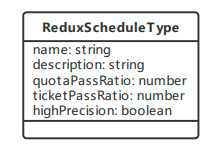
\includegraphics[height=3cm]{scheduleType.png}
    \caption{议程类型数据结构示意图}
    \label{fig:scheduleType}
  \end{figure}

  对于金额通过比例,若比率为负数,则意味着 “金额通过” 不考虑,对于精度到表决组的议程,该比率为 “各个表决组内通过金额” 的比率,对于精度到议程的议程,该比率为 “整个议程通过的金额” 的比率。

  对于票数通过比例,若比率为负数,则意味着 “票数通过” 不考虑,对于精度到表决组的议程,该比率为 “各个表决组内通过票数” 的比率,对于精度到议程的议程,该比率为 “选择通过的总债权人户数” 的比率。

  highPrecision (是否高精度)为计算精度。为 true 则意味着为高精度议程,即议程通过需要精确到各个表决组都通过,为 false 则意味着计算精度不高,只要议程下的总量数据通过即可,忽略表决组因素。另外,该字段会影响数据在前端的展示,目前只有 “重整计划” 议程是高精度的。

    \begin{figure}[!htp]
      \centering
      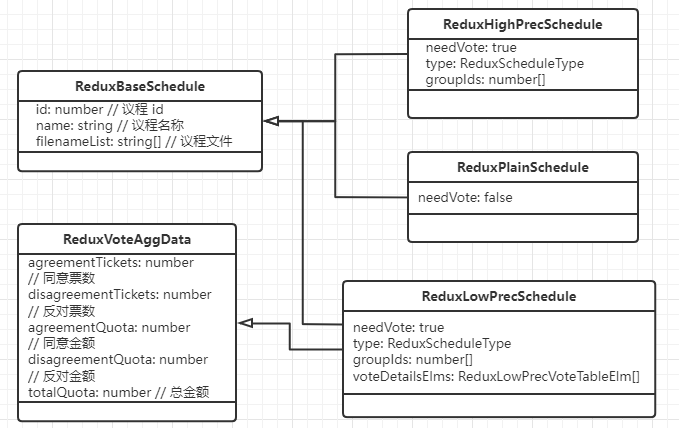
\includegraphics[height=10cm,width=14cm]{schedule.png}
      \caption{议程相关数据结构示意图}
      \label{fig:schedule}
    \end{figure}

    如图~\ref{fig:schedule}所示,对于表决议程来说,表决议程分为三种类型 highPrecSchedule (高精度表决议程)、lowPrecSchedule (低精度表决议程) 和 plainSchedule (普通议程)。以上三种类型议程均继承自 basicSchedule (基础议程), 基础议程中包含议程的ID号,议程的名称和议程的文件信息 (目前议程文件默认只有一个文件,即首文件)。

  plainSchedule (普通议程)即无需投票的议程,因此只在 basicSchedule (基础议程) 基础上多出了 needVote 属性,且值为 false,表示 plainSchedule (普通议程) 为无需投票的议程。

  highPrecSchedule (高精度表决议程) 即需要投票且投票精度到表决组级别的议程,在 basicSchedule (基础议程) 基础上多出了 needVote,type 和 groupIds 属性。needVote的值一定为 true,type 中 highPrecision 属性一定为 true, groupIds 用来存储和议程相关的所有表决组的ID号,高精度议程表决精确到表决组级别,因此 VoteAggData (表决复合数据) 在 group 级别。

  LowPrecSchedule (低精度表决议程) 即需要投票且投票精度到议程级别的议程,在 basicSchedule (基础议程) 基础上多出了 needVote,type,voteDetailsElms 和 groupIds 属性。needVote的值一定为 true,type 中 highPrecision 属性一定为 false, groupIds 用来存储和议程相关的所有表决组的ID号,voteDetailsElms 是低精度议程中,用于渲染 “表决详情” 的数据结构,每一项事实上是一个 meetingCreditor。低精度议程表决精确到议程级别,因此 VoteAggData (表决复合数据) 也在议程级别。

  VoteAggData (表决复合数据) 包含议程或表决组的表决情况,包含 agreementTickets (同意票数), disagreementTickets (反对票数), agreementQuota (同意金额), disagreementQuota (反对金额), totalQuota (总金额) 属性,用于展示议程或表决组的表决情况以及用于计算通过情况。

  \begin{figure}[!htp]
    \centering
    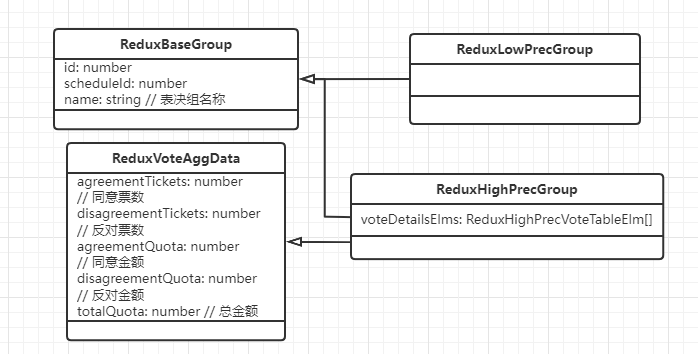
\includegraphics[height=8.5cm, width=14cm]{group.png}
    \caption{表决组相关数据结构示意图}
   \label{fig:group}
  \end{figure}

  如图~\ref{fig:group}所示,对于表决组来说,表决组分为两种类型 highPrecGroup (高精度表决组) 和 lowPrecGroup (低精度表决组) 。以上两种类型议程均继承自 basicGroup (基础表决组), 基础表决组中包含表决组的ID号,表决组的名称和表决组所属的议程ID。

  对于highPrecGroup (高精度表决组) 来说,由于高精度议程表决精确到表决组级别,因此VoteAggData (表决复合数据) 也在表决组级别,另外还包含 voteDetailsElms 属性,高精度议程中,用于渲染 “表决详情” 的数据,每一项事实上是一个 ticket。高精度下,各表决组 “总票数” 为该 map 的 size 大小。

  对于lowPrecGroup (低精度表决组) 来说,由于低精度议程会忽略表决组级别,因此低精度表决组只需保存基础表决含有的信息即可。

  \section{其他设计}
  在原本的设计中,会议页面中所有的 view state (视图状态)散落于各个组件内部,各个组件用到了表决服务的各种数据,其请求方法离散地分布在各个组件内部,这会让实时表决服务接入时发生以下问题:

  \quad{}a. 实时表决的 client scaffold (客户端支架)并非 useHooks 风格,实际上是 class,其所有的后端请求型数据对应的 handler 必须在该 class 初始化时设定好,且无法接受后续状态更新。也就是说,如果现有的组件保持原样,所有的组件都需要传入一个 realtimeUpdate 函数,在管理人会议页面中将至少 11 个函数组合在一起,置入 handler 中,以便于在表决后端传来请求型消息时更新各级子组件内部的 state,这会让代码非常不直观,难以维护。

  \quad{}b. 由于获取到的 client 生命周期很有可能是未准备好甚至已结束的,而 client 并非 useHooks 实现,各级子组件每次 state update 时并不会重新获取 client scaffold 的实体,而是保留老的引用。这很可能导致由部分组件由于加载的异步性,永远无法接收到后端传来的数据,也无法向后端发送数据。

  \quad{}c. 本系统前端要根据当前是否在实时表决的信息来让各个子组件的请求决定走向 SpringBoot后端还是实时服务。这个状态在各个子组件中分别做判断和共享非常麻烦且很容易遗漏,无论是 试用 redux 还是 context 或者将这个 state 以 props 传给所有人,都要进行大量的编码。这意味着,即使用 useHooks 实现 client scaffold,也难以保证目前组件状态更新的健壮性和可维护性。

  基于以上的考虑,本系统进行了前端组件的表决状态提升设计,即将管理人与债权人的会议页面下表决组件的各级子组件状态提升至父组件,使数据流更新清晰明了,具体实现如图~\ref{fig:state}所示。

  \begin{figure}[!htp]
    \centering
    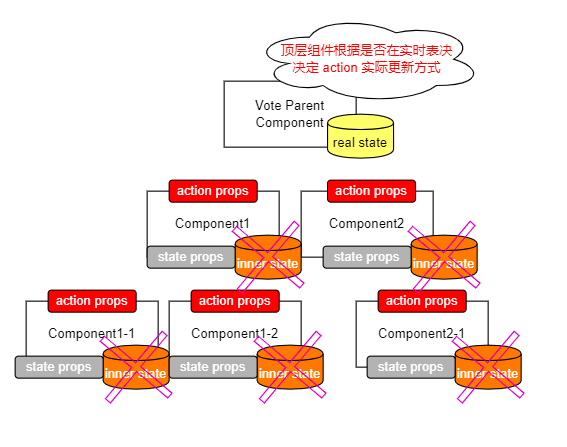
\includegraphics[height=8cm]{state.png}
    \caption{表决状态提升示意图}
   \label{fig:state}
  \end{figure}

  最顶层的组件中存有所有组件需要的真正 state,在上图中为亮黄色,数据为 SpringBoot后端 和 实时表决端拿到的复合数据。

  对于各级子组件,如果有表决相关的内部 state,将其定义为 inner state,全部删除。

  对于需要向后端请求数据的组件,将这个函数定义为 action,将它作为 props,由顶层组件级级传入。这意味着这部分数据的更新让顶层组件决定。action props 在图中显示为鲜红色。

  对于完全由 real state 决定的 state,直接将其作为 props 传入即可。这部分 props 在图中为深灰色。

对于实时表决时期,real state 只在第一次 action 触发时向 SpringBoot 后端获取数据,接下来这些 real state 都会接受实时数据的更新,

对于非实时表决时期,所有的 action 都将被设定为跳过从实时表决后端获取实时数据,直接从 SpringBoot 后端获取数据。

\section{本章小结}
本章首先介绍了前端两个重要的特殊设计。一是因为在管理人部分系统前端已有全量的数据存在,对于表决结果的计算放在前端会更快捷,也可以减少后端的压力。因此在前端维护了一套数据库,用与存储会议相关的全量数据和进行表决结果计算。第一小节具体介绍了前端数据库的设计。二是由于前端不同表决类型议程的渲染逻辑区分复杂,为了使渲染代码逻辑更加清晰,在前端提出了一层新的抽象:表决计算精度,通过加入表决计算精度,使业务代码可维护性变强了,也使得前端渲染逻辑更加清晰。另外,本章第三小节详细介绍了前端在上述两个特殊设计的情况下,Redux 中相关的数据结构设计。最后本章介绍了在前端设计中遇到的一些其他问题以及解决方法。
% !TeX root = ../main.tex

\chapter{实验设计}

\section{系统功能性测试}
在系统进入内测阶段,我们对系统进行了功能性测试。按照需求说明书的标准,我们测
试了系统的所有功能。图~\ref{fig:test1} 是系统功能性测试用例表。用例表是测试上传表决数据的测试用例。

\begin{figure}[!htp]
    \centering
    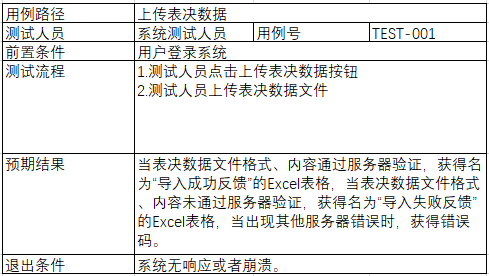
\includegraphics[height=5cm]{test1.png}
    \caption{测试用例表}
    \label{fig:test1}
  \end{figure}

  表~\ref{fig:test2}是我们进行功能性测试的结果。严重错误是指用户操作完系统无响应,系统发生了崩溃;而普通错误主要指在人机交互中的出错;而小错误则是一些显示上的字段错误或
  者页面编排上的小错误。在每次测试迭代过程中,我们都按照上一轮测试的结果不断进行
  修正,不断优化系统。

  \begin{table}[h!]
    \begin{center}
      \caption{系统功能性测试结果}
      \label{fig:test2}
      \begin{tabular}{ c c c c }
        \hline
        \textbf{测试轮数} & 1 & 2 & 3 \\
        \hline
        \textbf{小错误} & 28 & 5 & 0 \\
        \textbf{普通错误} & 20 & 2 & 0 \\
        \textbf{严重错误} & 5 & 1 & 0 \\
        \hline
      \end{tabular}
    \end{center}
  \end{table}

\section{系统性能测试}
在满足功能需求的前提下,我们需要保证系统的性能需求。本节性能测试将主要介绍三个测试,一是前端组件更新性能测试,二是 Mongo 写入性能测试,三是集群 Kafka 订阅发布性能测试。

\subsection{前端组件更新性能测试}
前端测试通过使用 immutable.js 写出测试页面,测试页面包含一个 table,通过脚本生成数据,更新数据并计算平均消耗时间,测试页面如图~\ref{fig:test3}。

\begin{figure}[!htp]
    \centering
    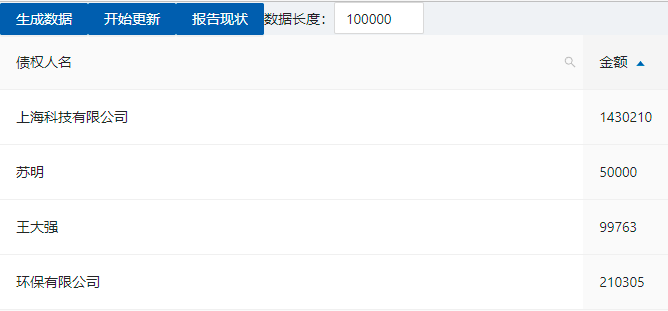
\includegraphics[height=6cm]{test3.png}
    \caption{前端测试页面}
    \label{fig:test3}
  \end{figure}

  为了测试前端在使用了 immutable.js 后,在 10000 条数据的情况下平均每条数据的更新所需时间,在测试页面输入数据长度为 10000,点击生成数据并点击开始更新,等待一段时间后点击报告现状,得到平均更新所需时间如如图~\ref{fig:test4},在表格 10000 条数据的情况下,平均更新每条信息所花费的时间为 18.73 ms,可以满足需求。

  \begin{figure}[!htp]
    \centering
    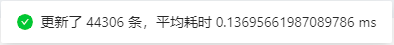
\includegraphics[height=2cm]{test4.png}
    \caption{前端测试结果}
    \label{fig:test4}
  \end{figure}

  \subsection{Mongo 写入性能测试}
  本文使用 Jmeter 测试工具进行了性能测试,测试了 Mongo 集群的写入性能。创建一个测试接口,此测试接口仅含有一次写入 Mongo 操作,通过 Jmeter 测试工具提升并发量,查看平均响应时间和 P95 响应时间,表~\ref{fig:test5}是我们进行测试的结果。根据性能测试的结果,可以推算出 Mongo 仅支持 700+ QPS,在高并发系统中明显为性能瓶颈。
  \begin{table}[h!]
    \begin{center}
      \caption{系统功能性测试结果}
      \label{fig:test5}
      \begin{tabular}{ c c c c }
        \hline
        \textbf{并发量} & \textbf{平均响应时间(ms)
        } & \textbf{P95值(ms)
        } & \textbf{P95平均值(ms)
        } \\
        \hline
        50 & 105 & 157 & 102 \\
        100 & 116 & 194 & 112 \\
        200 & 165 & 300 & 157 \\
        300 & 264 & 418 & 255 \\
        400 & 295 & 510 & 279 \\
        500 & 724 & 1007 & 702 \\
        600 & 864 & 1264 & 840 \\
        700 & 971 & 1559 & 937 \\
        800 & 1032 & 1584 & 997 \\
        900 & 1215 & 1864 & 1171 \\
        \hline
      \end{tabular}
    \end{center}
  \end{table}

  \subsection{Kafka 订阅发布性能测试}
  本视频表决会议系统作为高并发系统,可能存在短时间内请求过多使服务器服务宕机的情况,可能出现高并发情况的功能有实时表决和实时聊天,如果在短时间内大量债权人同时投票则实时表决会在短时间内出现大量请求,实时聊天同理,由于并发都是针对于实时性的功能,性能瓶颈需要考虑实时 WebScoket 端性能和 Mongo 的写入性能,而前面测试得到 Mongo 的写入性能无法满足系统的要求,为系统的性能瓶颈,仅仅通过增加服务实例的方式无法解决请求过多的情况,因此在 WebSocket端还需要进行流量削峰,本系统使用消息中间件 Kafka 达到流量削峰的目的,本节将测试 Kafka 订阅发布的性能,来确认 Kafka 的性能是否满足要求,是否会成为系统的性能瓶颈。

  测试在 100 个分区,1 个订阅的情况下测试订阅发布的延迟,结果表~\ref{fig:test6},所示。当ack=1,消息被追加到leader副本所在分区后再确认,当ack=all,在所有的ISR(同步副本)都接收到消息时才确认,在这两种情况下,平均响应时间为 4+ ms,能够满足系统需求。

  通过对 Mongo 写入性能的测试和对 Kafka 订阅发布性能的测试结果进行对比后发现,可以确定本系统性能瓶颈为 Mongo 写入性能,因此后续出现性能瓶颈时需要考虑对系统 Mongo 的写入性能进行优化。

  \begin{table}[h!]
    \begin{center}
      \caption{系统功能性测试结果}
      \label{fig:test6}
      \begin{tabular}{ c c c c }
        \hline
        \textbf{类型} & \textbf{平均响应时间(ms)
        } & \textbf{P90值(ms)
        } & \textbf{P99值(ms)
        } \\
        \hline
        Kafka-ack-1 & 4.26 & 5.39 & 6.94 \\
        Kafka-ack-all & 4.22 & 5.19 & 10.43 \\
        \hline
      \end{tabular}
    \end{center}
  \end{table}
% !TEX root = ../main.tex

\chapter{全文总结}
本章将对支持大规模高并发、实时反映表决情况的债权人会议系统的设计与实现的工作进行总结,并根据课题论文的研究成果展望该领域未来发展方向。

本次课题研究以法律业务数字化为基点开展了研究,并且设计了针对高并发、实时反映表决情况的债权人会议系统,解决了债权会议业务数字化的问题,使债权会议全面线上化。在具体研究的过程中,所涉及到的开发技术有:面向对象程序设计、网页制作技术、消息队列、高速缓存等,最终设计并实现了高并发债权人会议系统。具体研究内容有:

1. 通过与甲方律师不断商讨的方式了解用户对于债权人会议系统的需求。对于实际需求,采用软件工程需求描述语言确定了系统的功能性需求。明确了软件开发的目标和开发的标准。

2. 针对高并发债权人会议系统的设计工作。为了适应本系统的需求,设计了针对性的架构解决系统性能问题。

3. 系统的开发及测试分析。概述了系统的前后端具体设计和部分实现。展示核心功能功能
的运行界面。完成系统设计之后,对系统进行功能性测试和部分性能测试。

本系统是对传统行业产业数字化的一次尝试。通过将信息技术应用于传统法律行业,系统
帮助实现破产领域债权会议业务的数字化,极大提高了债权会议业务的进行效率。当然
系统本身也存在一些不足之处,比如系统的 Mongo 写入性能为本系统的性能瓶颈,若后续系统达到性能瓶颈,需要对 Mongo 的写入性能做出优化。



%TC:ignore

% 参考文献
\printbibliography[heading=bibintoc]

% % 附录
% \appendix

% % 附录中图表不加入索引
% \captionsetup{list=no}

% % 附录内容
% \input{contents/app_maxwell_equations}
% \input{contents/app_flow_chart}

% 结尾部分
\backmatter

% 用于盲审的论文需隐去致谢、发表论文、科研成果、简历

% 致谢
% !TEX root = ../main.tex

\begin{acknowledgements}
  感谢上海交通大学软件学院高质量的教学水平,开设诸多高质量的专业课,让我有机会在大学四年的时光中系统地学习计算机基础和软件工程等方面地知识,并能从事相关开发实践。在软件学院诸多优秀的老师和同学的陪伴下,我大学四年受益良多。

  感谢吴刚老师和任锐老师在我编写本论文过程中的指导。老师们在系统开发方面丰富的实
  践经历和全面的系统意识让我受益良多,他们严谨认真的科研精神也在时时刻刻地给予我正面的影响。通过和老师们的交流,我进一步学习了软件工程开发思想和软件系统架构设计的相关知识。感谢老师们能够在我在进行本课题研究遇到问题和疑惑时及时向我伸出援手。

  感谢 SAIL 实验室的林许亚伦学长和郑宇宸学长在我开发系统过程给予我的帮助。学长
  们十分热心负责,在开发过程中提出了非常多有用的建议,并且协助我解决了很多难题,他们的工作态度令人敬佩。

  感谢软件工程专业的蒋钊、龙泓杙两位同学这四年以来的帮助和陪伴。两位同学发现问题提出问题的能力,解决问题严谨认真的态度对我影响颇大,并且在学业和项目方面对我帮助颇多,在此对他们由衷的感谢。
\end{acknowledgements}


% % 发表论文及科研成果
% % 盲审论文中,发表论文及科研成果等仅以第几作者注明即可,不要出现作者或他人姓名
% \input{contents/achievements}

% % 简历
% \input{contents/resume}

% 学士学位论文要求在最后有一个大摘要,单独编页码
% !TEX root = ../main.tex

\begin{digest}
  Digitalization is the advanced stage of the development of information technology and the main driving force of digital economy. With the rapid development of the new generation of digital technology, all walks of life create more and more value by using digital technology, which promotes all walks of life to accelerate the digital transformation.



The digitalization mentioned in this paper mainly refers to the digital transformation of specific business and scene by using digital technology. The digital technology revolution has promoted the digital transformation of mankind. The economy of human society with the progress of technology evolved, farming technology opens the agricultural economy, industrial revolution to realize the evolution of the agricultural economy to industrial economy, now the digital technology revolution, to promote the digital revolution of human production and living, gives birth to a new economic form - digital economy, digital driving force to become the core of the digital economy. The continuous improvement of digital technology gives full play to the value of digitalization. In recent years, various digital technologies such as the Internet of Things, cloud computing and artificial intelligence have been constantly updated and gradually industrialized from experiment to practice, forming a complete digital value chain that has been applied in various fields, promoting the digitalization of various industries and creating new values for all industries. The rapid development of digital infrastructure drives the adoption of digitization. In recent years, China has been accelerating the construction of digital infrastructure, promoting the integrated innovation and application of industrial Internet, artificial intelligence, Internet of Things, Internet of vehicles, big data, cloud computing, block chain and other technologies, so as to make digital application more widely and deeply into all levels of social and economic operation and promote the development of digital economy.



As a traditional industry, the lawyer industry is still in the traditional handicraft era. Information is collected and sorted out by paper materials and stored in warehouses, which greatly affects efficiency. At present, in the midst of the epidemic, offline work is greatly restricted, and business will not be reduced because of the existence of restrictions. A large amount of business accumulation has brought great inconvenience, and the digital reform of the lawyer industry is imminent.



In the field of bankruptcy, the significance of meeting and voting is very important, which determines the trend of a bankruptcy project. In order to realize the digital transformation of bankruptcy business, it is essential to design a meeting system for bankruptcy project voting. Creditors of enterprise bankruptcy project are easy to reach the level of thousands or even ten thousand. If multiple meetings are held at the same time and voting is conducted in the same period, the concurrency will be greatly increased, causing great pressure on the server. Therefore, it is necessary to design and develop a meeting voting system specifically for high concurrency.



The research significance of comprehensive digitalization of creditor's rights meeting in the field of bankruptcy mainly includes the following three points:

One is that due to the COVID-19 pandemic, holding creditors' meetings online has become the main choice of managers. The advantages of online operation of bankruptcy cases represented by the network creditors' meeting are very obvious -- this advantage is not only reflected in the epidemic period, online operation is more convenient, fast, standardized and efficient in both program design and equipment use, and represents the future work trend of bankruptcy business. Network creditor's meeting is an innovation of the way of holding creditor's meeting by using network technology in the network era, which is conducive to improving work efficiency and better protecting creditor's rights. However, the network creditors' meeting is different from the traditional creditors' meeting, and many new problems need to be solved. Creditor's rights conference system is different from the conventional conference system, which is closely linked with the bankruptcy law. The conventional conference system is not applicable, so it is necessary to design and develop a targeted creditor's rights conference system.



Second, digitalization takes data as the main factor of production, converts all valuable people, things and things in the enterprise, such as business, production, marketing and customers, into digital stored data, forming data, information and knowledge that can be stored, calculated and analyzed. Together with external data obtained by the enterprise, Through the real-time analysis, calculation and application of these data can guide enterprises' production, operation and other businesses. And each creditor's rights meeting can produce a large amount of data, which can produce great economic value, so it is necessary to ensure the reliability of the storage of these data.



Third, with the rapid rise of computer technology and network technology in recent years, the Internet is changing people's way of production and life. The development of the Internet has brought about a surge in demand and pressure on technology, so the system architecture is constantly evolving, upgrading and iterating. From single application, to vertical split, to distributed services, to SOA, and now the hot microservices architecture. Although most of the problems have been solved, there are still some problems even when the traffic volume is relatively large, especially high concurrency and high availability still need a lot of design and research. For creditor's rights conference system, a creditor meeting is usually one thousand to ten thousand the number of levels, some even reach one hundred thousand level, if for many meetings at the same time, and meeting voting is usually concentrated in a period of time, that leads to the high concurrency issues, and the creditor meeting data very important, if the loss of important data or service suddenly lockout, Therefore, in the process of digitalization of creditor's rights meeting, the importance of targeted design with high concurrency and high availability is self-evident.



The main work of this thesis is the design and implementation of high concurrent video voting conference system. This topic will study how to design a system to meet the needs of legal cases of bankruptcy reorganization creditor's rights meeting and how to achieve it. The main research contents include the architecture design of the debt conference system in high concurrency scenario, the data storage design of the debt conference system in high concurrency scenario, the high availability of database in high concurrency scenario, and the front-end design and optimization of the debt conference system. The main work content is the creditor's rights conference system design and the creditor's rights conference system front and back end development and performance test.
\end{digest}


%TC:endignore

\end{document}
